\documentclass[11pt,reqno]{amsart}
\usepackage[margin=1.15in]{geometry}
\usepackage{amsmath,amssymb,amsthm,mathtools}
\usepackage{graphicx}
\usepackage{booktabs}
\usepackage[colorlinks=true,linkcolor=blue,citecolor=blue,urlcolor=blue]{hyperref}
\usepackage{microtype}
\usepackage{xurl}
\raggedbottom

\theoremstyle{plain}
\newtheorem{theorem}{Theorem}
\newtheorem{proposition}[theorem]{Proposition}
\newtheorem{corollary}[theorem]{Corollary}
\newtheorem{lemma}[theorem]{Lemma}
\newtheorem{conjecture}[theorem]{Conjecture}
\theoremstyle{definition}
\newtheorem{definition}[theorem]{Definition}
\newtheorem{remark}[theorem]{Remark}
\newtheorem{observation}[theorem]{Observation}

\DeclareMathOperator{\sqf}{sqf}
\newcommand{\Art}{\mathrm{Art}}
\newcommand{\Acal}{\mathcal{A}}
\newcommand{\Z}{\mathbb{Z}}
\newcommand{\Q}{\mathbb{Q}}
\newcommand{\Lsym}[2]{\left(\tfrac{#1}{#2}\right)}
\newcommand{\E}{\mathbb{E}}

\begin{document}

%% ===================== NEW FRONT MATTER (consolidated paper) =====================
\title[Correlations of Artin status among primes]{Correlations of Artin status among primes:\\ consecutive-prime anticorrelation, cross-base entanglement,\\ and an elementary decomposition}

\author{Josh Bald}
\address{Ontario, Canada}
\email{jpbald93@gmail.com}
\thanks{\textbf{Corresponding author.} Josh Bald, Independent Researcher.
	Email: \texttt{jpbald93@gmail.com}. ORCID: \texttt{0009-0002-1317-6489}.}

\subjclass[2020]{Primary 11A07; Secondary 11N05, 11N13, 11Y16, 11Y60}
\keywords{Artin's primitive root conjecture, primitive roots, consecutive primes,
	Lemke Oliver--Soundararajan bias, entanglement, quadratic characters,
	Legendre symbol, full reptend primes, computational number theory}

\date{September 2026}

\begin{abstract}
	Say a prime $p$ is \emph{Artin base $a$} if $a$ is a primitive root modulo $p$.
	This paper studies correlations of Artin status along two axes --- \emph{consecutive
	primes} at a fixed base, and \emph{several bases} at a fixed prime --- for all primes up to $10^9$ (with $50{,}847{,}531$ of them, $p\ge 7$, in the
	consecutive census), and then asks what, if anything, such correlations are
	computationally worth.

	Along the first axis, Artin statuses of consecutive primes are measurably
	\emph{anticorrelated} at base $10$: $P(\Art_{n+1}\mid\Art_n)=0.36514$ against
	$P(\Art_{n+1}\mid\lnot\Art_n)=0.37928$, a deficit $\delta=-0.01414$
	(Pearson $10{,}167$ on one degree of freedom; signed square root $-100.8$ under a
	nominal independent-status reference, over $50{,}847{,}530$ pairs). The dependence
	has strong gap structure and contains one deterministic component, an elementary
	\emph{exclusion law}: if $p,p+g>5$ are prime with $g\equiv 20 \pmod{40}$, then $10$
	is a quadratic residue modulo exactly one of them, so the two can never both be
	Artin; among $2{,}195{,}882$ pairs at gaps $20$ and $60$ there is no doubly-Artin
	pair, and an independent recomputation extends this to $194{,}296{,}748$ such pairs
	below $10^{11}$, again with none. Conversely $g \equiv 0 \pmod{40}$ forces equal
	quadratic-residue status and strong positive dependence ($P(\Art_{n+1}\mid\Art_n)=0.899$
	at $g=40$). Conditioning on the joint residues of $(p_n,p_{n+1})$ modulo $120$ or
	$840$ places $98.7\%$ and $99.5\%$ of the global deficit between joint-residue cells
	rather than within them (an exact covariance decomposition; $96.1$--$99.2\%$ and $97.8$--$99.7\%$
	across the four weighting conventions we report). As an intermediate link we report the apparently unreported
	anticorrelation $r(\omega(p_n-1),\omega(p_{n+1}-1))=-0.041$.

	Along the second axis we record a second exclusion law: writing $d=\sqf(ab)$ for the
	squarefree part of $ab$, no prime with $\bigl(\tfrac{d}{p}\bigr)=-1$ is simultaneously
	Artin for $a$ and for $b$; whenever $a$ and $b$ have different squarefree parts this
	bars half of all primes, and it implies a triple form --- if $\sqf(c)=\sqf(ab)$ then no
	odd prime is Artin for $a,b,c$ at once (e.g.\ $2,5,10$). Across the $66$ base pairs of
	$\{2,3,5,6,7,10,11,13,15,17,21,29\}$ the measured same-prime correlation $\phi(a,b)$ is
	positive for $64$ pairs (mean $0.0352$); conditioning on $\omega(p-1)$ removes only
	$55\%$ of it, while conditioning on a fine signature of $p-1$ removes $95\%$. The
	residual is concentrated on the fifteen pairs whose product class completes a triple
	and lies in the quadratic-character channel. Joint densities predicted by the
	Matthews--Moree--Stevenhagen Kummer-degree heuristic match the measured densities to a
	mean relative error of $0.012\%$ with no fitted parameters.

	Finally we \emph{audit the computational content} of these correlations. In a resubstitution diagnostic the consecutive-prime correlation carries $0.000009$ nats
	($1.3\times10^{-5}$ bits) of conditional-entropy reduction beyond the elementary
	joint-residue baseline, which itself carries $0.4195$ nats. A simulation in which every
	status depends only on $p \bmod 840$ reproduces the part of that increment which exceeds
	the mod-$120$ baseline: it is residue information (the prime $7$ of $p-1$), not information
	carried by the predecessor's status, and in held-out scoring the predecessor's status
	gives no gain beyond residues mod $840$.
Both exclusion laws are computationally redundant: the gap law from quadratic reciprocity
	together with multiplicativity, the same-prime law from multiplicativity alone. The one genuinely usable filter --- a primitive root must be a
quadratic non-residue --- is elementary, is exactly what the observed conductor-$40$
channel expresses, and halves the factorizations of $p-1$ in a scanning search; ordering
	the small prime channels of $p-1$ before the full factorization is about $13\%$ faster
	again.
We conclude that these correlations describe arithmetic structure rather than supply
algorithms, and we state precisely what would have to change for that verdict to change.
\end{abstract}

\maketitle

\section{Introduction}
\label{sec:intro}

Artin's conjecture on primitive roots, communicated to Hasse in 1927 (see
\cite{Artin1965}), concerns one base at a time: for non-square
$a \ne 0, \pm 1$ the set of primes $p$ for which $a$ is a primitive root mod $p$
should have positive density, a multiple of Artin's constant
$C = \prod_q \bigl(1 - \tfrac{1}{q(q-1)}\bigr) \approx 0.3739558$; for base $10$ no
correction factor applies, so the conjectural density is exactly $C$. Hooley~\cite{Hooley1967}
proved this under GRH; unconditionally, Gupta--Murty~\cite{GuptaMurty1984} and
Heath-Brown~\cite{HeathBrown1986} showed the conjecture can fail for at most two prime
bases, and Klurman--Shparlinski--Ter\"av\"ainen~\cite{KlurmanShparlinskiTeravainen2025}
established the predicted asymptotic on average over almost all small bases; recent work
has sharpened the analytic understanding for individual primes, with Fan and Pollack
\cite{FanPollack2025} proving a version uniform in the base and Perucca and Shparlinski
\cite{PeruccaShparlinski2025} giving uniform upper and lower bounds for the Artin density.
Moree's survey~\cite{Moree2012} is the standard account. For $a=10$ the property has a classical
meaning: $10$ is a primitive root mod $p$ exactly when the decimal expansion of $1/p$ has
maximal period $p-1$ --- the \emph{full reptend} primes~\cite[pp.~166--171]{ConwayGuy1996}.

Three further strands meet here. The first is the bias discovered numerically by
Knapowski--Tur\'an, Ko and Ash--Beltis--Gross--Sinnott and quantitatively treated by
Lemke Oliver and Soundararajan~\cite{LOS2016}: consecutive primes in the same reduced
residue class modulo $q$ occur markedly less often than equidistribution predicts, a
phenomenon explained conjecturally by the Hardy--Littlewood $k$-tuple
conjectures~\cite{HardyLittlewood1923}. Since the Artin property of $p$ is governed by the
factorisation of $p-1$, and since residues of consecutive primes modulo small $q$ are
correlated by~\cite{LOS2016}, one expects \emph{some} induced dependence between the Artin
indicators of consecutive primes. The second is the joint behaviour \emph{across bases} at
a fixed prime, computed under GRH by Matthews~\cite{Matthews1976} and systematically by
Moree--Stevenhagen~\cite{MoreeStevenhagen2014}, with the qualitative message that
$\Acal_a$ and $\Acal_b$ are \emph{not} independent and that the deviation is governed by
entanglement of the associated Kummer--Galois extensions. The framework remains active:
Lenstra's Galois-theoretic setting~\cite{Lenstra1977}, the unified Artin-type treatment of
J\"arviniemi--Perucca--Sgobba~\cite{JarviniemiPeruccaSgobba2025}, unconditional results in
cases where GRH can be circumvented~\cite{Sgobba2025}, and number-field variants
\cite{Kimmel2024}. The third is the question of
which primes at a fixed shift can \emph{both} be Artin: Tinkov\'a--Waxman--Zindulka
\cite{TinkovaWaxmanZindulka2023} identify shift--base pairs admitting no such prime, and
our Theorem~\ref{thm:exclusion} is the base-$10$ instance of that phenomenon; we claim no
priority for it.

The present paper asks the \emph{statistical} question along both axes --- how Artin
statuses of consecutive primes are correlated on average, and how Artin statuses of several
bases are correlated at the same prime --- and then asks a question we have not seen posed
in this literature: \emph{what is such a correlation computationally worth?}\footnote{An
earlier version of parts of this work appeared as the preprints \emph{Correlations between
primitive root statuses of consecutive primes} (Zenodo,
\href{https://doi.org/10.5281/zenodo.22863946}{doi:10.5281/zenodo.22863946}) and
\emph{Cross-base correlations of Artin primes} (Zenodo,
\href{https://doi.org/10.5281/zenodo.22878204}{doi:10.5281/zenodo.22878204}). This paper
consolidates those two preprints and adds the audit of \S\ref{sec:content}; it supersedes
them, and the preprints are retained for the record.} The answer we give is a measured
negative, and we regard it as part of the result rather than a failure of it.

Two comparisons should be made explicit. Garcia--Kahoro--Luca~\cite{GarciaKahoroLuca2019}
(see also~\cite{GarciaLucaShiUdell2020}) compare the \emph{number} of primitive roots,
$\varphi(p-1)$ versus $\varphi(p+1)$, for twin pairs; Pollack~\cite{Pollack2014} and
Baker--Pollack~\cite{BakerPollack2016} prove existence of runs of consecutive primes each
having a prescribed primitive root. Those are existence results, produced by sieves that
select rare favourable configurations; they say nothing about the typical joint behaviour
along the sequence of primes. The questions studied here are complementary: the average
correlation, its decomposition, and its computational content.

\section{Summary of results}
\label{sec:summary}

Throughout, \emph{Artin prime} means Artin prime for base $10$ unless stated otherwise,
$p_n$ denotes the $n$-th prime, $\omega(m)$ the number of distinct prime factors of $m$,
and $\sqf(m)$ the squarefree part of $m$.

\begin{enumerate}
	\item \textbf{Consecutive-prime exclusion law} (Theorem~\ref{thm:exclusion}). If $p$ and
	$p+g$ are primes with $p,p+g>5$ and $g\equiv 20 \pmod{40}$, then
	$\Lsym{10}{p+g}=-\Lsym{10}{p}$; consequently at most one of the two is Artin base $10$.
	If instead $g\equiv 0 \pmod{40}$ then $\Lsym{10}{p+g}=\Lsym{10}{p}$.
	\item \textbf{Same-prime exclusion law} (Theorem~\ref{thm:pair}). With $d=\sqf(ab)$, no
	prime with $\Lsym{d}{p}=-1$ is Artin for both $a$ and $b$. If $\sqf(c)=\sqf(ab)$ then no
	odd prime is Artin for $a$, $b$ and $c$ simultaneously (Theorem~\ref{thm:triple}).
	\item \textbf{Consecutive-prime anticorrelation} (\S\ref{sec:global}). Across all
	$50{,}847{,}530$ consecutive pairs up to $10^9$,
	$\delta = P(\Art_{n+1}\mid\Art_n)-P(\Art_{n+1}\mid\lnot\Art_n) = -0.01414$, with
	Pearson $\chi^2 = 10{,}167$ on one degree of freedom.
	\item \textbf{Gap structure} (\S\ref{sec:gaps}). $\delta(g)$ ranges from $-0.592$ at
	$g=60$, where the theorem forces exclusion, to $+0.643$ at $g=40$.
	\item \textbf{Residue conditioning} (\S\ref{sec:decomposition}). Conditioning on the
	joint residues of $(p_n,p_{n+1})$ modulo $120$ and $840$ gives an exact covariance
	decomposition of the global deficit, placing $98.69\%$ and $99.55\%$ of it between cells
	(within-cell terms $-0.000186$ and $-0.000064$); across four weighting conventions the
	between share lies in $[96.1\%,99.2\%]$ and $[97.8\%,99.7\%]$.
	\item \textbf{$\omega$ repulsion} (\S\ref{sec:omega}).
	$r(\omega(p_n-1),\omega(p_{n+1}-1)) = -0.0410$.
	\item \textbf{Cross-base correlation} (\S\ref{sec:measurement}). Over the $66$ pairs of
	the base set, $\phi(a,b)$ is positive for $64$ pairs (mean $0.0352$); the only negative
	pairs are $(2,10)$ and $(3,15)$.
	\item \textbf{Decomposition of the cross-base correlation} (\S\ref{sec:decomposition_crossbase}).
	Conditioning on $\omega(p-1)$ removes $55\%$ of the mean signed correlation; conditioning
	on the fine signature $\mathrm{sig}(p)$ removes $95\%$ of it.
	\item \textbf{Residual localisation} (\S\ref{sec:entanglement}). The surviving residual
	is concentrated on the triple-completing pairs and lies in the quadratic-character
	channel.
	\item \textbf{Kummer-degree densities} (\S\ref{sec:model}). The
	Matthews--Moree--Stevenhagen predictions match the measured joint densities to a mean
	relative error of $0.012\%$, with no fitted parameters.
	\item \textbf{Computational content: a measured negative} (\S\ref{sec:content}). The
	consecutive-prime correlation adds $0.000009$ nats of in-sample conditional-entropy
	reduction to the mod-$120$ joint-residue baseline; a residue-only simulation shows that
	excess to be residue information mod $840$, and no held-out estimator we tested gains
	beyond residues mod $840$; both exclusion laws are computationally
	redundant, the same-prime law from character multiplicativity alone and the gap law from
	reciprocity together with it;
	the only usable filter is the elementary non-residue test, which the conductor-$40$
	channel expresses.
\end{enumerate}

\section{Preliminaries and notation}
\label{sec:prelim}

For an odd prime $p$ not dividing $a$, write $\Lsym{a}{p}$ for the Legendre symbol and
$\chi_a(p)=\Lsym{a}{p}$ for the quadratic character of conductor $\mathrm{cond}(\chi_a)$.
Write $\Acal_a$ for the set of primes for which $a$ is a primitive root, and
$X_a(p)=\mathbf{1}[\,p\in\Acal_a\,]$ for its indicator; along the consecutive-prime axis we
abbreviate $\Art_n = \mathbf{1}[\,p_n\in\Acal_{10}\,]$ for Artin status at the $n$-th prime.
Then $a$ is a primitive root modulo $p$ exactly when $a^{(p-1)/\ell}\not\equiv 1 \pmod p$ for every prime
$\ell \mid p-1$. Two elementary facts are used repeatedly. First, if $X_a(p)=1$ then
$\Lsym{a}{p}=-1$: a primitive root has order $p-1$, so $a^{(p-1)/2}\equiv -1$, whereas a
quadratic residue satisfies $a^{(p-1)/2}\equiv 1$. Second, quadratic characters are
multiplicative in the numerator, $\Lsym{ab}{p}=\Lsym{a}{p}\Lsym{b}{p}$, and the Legendre
symbol depends on $p$ only through $p \bmod 4d$ when $d=\sqf(ab)$.

The Artin property of $p$ is determined by the prime factorisation of $p-1$: the criterion
consults $\ell=2$ and every prime divisor $\ell$ of $p-1$. This is why both decompositions
below are stratified by the \emph{fine signature}
\[
	\mathrm{sig}(p) = \Bigl(\min(v_2(p-1),4),\;\; \{\,q\le 13 : q\mid p-1\,\},\;\;
	\min(\omega_{>13}(p-1),3)\Bigr),
\]
a partition of the primes into at most $4\cdot 32\cdot 4 = 512$ cells (for odd $p$ one has
$v_2(p-1)\ge 1$, so the truncated valuation takes four values, not five). The signature
is a coarse summary of the part of $p-1$ that the criterion consults first for small bases;
it records neither all prime divisors of $p-1$ nor the power-residue outcomes the criterion
tests, and so does not determine Artin status.



\section{The consecutive-prime exclusion law}
\label{sec:theorem}

\begin{definition}
	For an odd prime $p \nmid 10$, write $\Lsym{10}{p}$ for the Legendre symbol.
	We say $p$ is an \emph{Artin prime} (for base $10$) if the multiplicative order
	of $10$ modulo $p$ equals $p - 1$.
\end{definition}

If $10$ is a quadratic residue mod $p$ then its order divides $(p-1)/2$, so a
QR is never a primitive root; $\Lsym{10}{p} = -1$ is a necessary (not
sufficient) condition for the Artin property.

\begin{theorem}[Exclusion law for gaps $\equiv 20 \pmod{40}$; cf.\ {\rm\cite[Thm.~1.1]{TinkovaWaxmanZindulka2023}}]
	\label{thm:exclusion}
	Let $p$ and $p' = p + g$ be primes with $p, p' > 5$ and $g > 0$,
	$g \equiv 20 \pmod{40}$.
	Then
	\[
		\Lsym{10}{p'} = -\Lsym{10}{p}.
	\]
	In particular, $10$ is a quadratic residue modulo exactly one of $p, p'$, and
	at most one of them is an Artin prime for base $10$.
\end{theorem}

\begin{proof}
	By multiplicativity, $\Lsym{10}{p} = \Lsym{2}{p}\Lsym{5}{p}$.

	Since $g \equiv 0 \pmod 5$, we have $p' \equiv p \pmod 5$. By quadratic
	reciprocity ($5 \equiv 1 \bmod 4$), $\Lsym{5}{p} = \Lsym{p}{5}$ depends only on
	$p \bmod 5$; hence $\Lsym{5}{p'} = \Lsym{5}{p}$.

	Since $g \equiv 4 \pmod 8$, we have $p' \equiv p + 4 \pmod 8$. The map
	$r \mapsto r + 4$ on odd residues mod $8$ exchanges $1 \leftrightarrow 5$ and
	$3 \leftrightarrow 7$. By the second supplementary law,
	$\Lsym{2}{p} = +1$ iff $p \equiv \pm 1 \pmod 8$, and the exchange maps
	$\{1, 7\}$ onto $\{5, 3\}$ and vice versa; hence $\Lsym{2}{p'} = -\Lsym{2}{p}$
	for every admissible residue.

	Multiplying, $\Lsym{10}{p'} = -\Lsym{10}{p}$. Whichever of the two primes has
	$\Lsym{10}{\cdot} = +1$ satisfies $\operatorname{ord}(10) \mid (p-1)/2 < p-1$, so it
	is not an Artin prime.
\end{proof}

\begin{corollary}[Coupling law for gaps $\equiv 0 \pmod{40}$]
	\label{cor:coupling}
	If $p, p' = p + g$ are primes with $p, p' > 5$ and $g \equiv 0 \pmod{40}$, then
	$\Lsym{10}{p'} = \Lsym{10}{p}$. In particular, if either is an Artin prime,
	then $10$ is a quadratic non-residue for both.
\end{corollary}

\begin{proof}
	Now $g \equiv 0 \pmod 8$ and $g \equiv 0 \pmod 5$, so both
	$\Lsym{2}{\cdot}$ and $\Lsym{5}{\cdot}$ are preserved.
\end{proof}

\begin{remark}
	The modulus $40$ is specific to base $10$: it is the conductor of the
	quadratic character $p \mapsto \Lsym{10}{p}$, namely $4 \cdot 10 = 40$ (the
	discriminant of $\mathbb{Q}(\sqrt{10})$). For a general non-square integer base $a$
	the same argument applies with $40$ replaced by the conductor $|d_a|$ of the
	quadratic character attached to $\mathbb{Q}(\sqrt{a})$: for odd primes
	$p, p'$ with $p \nmid a$ and $p' \nmid a$, gaps
	$g \equiv 0 \pmod{|d_a|}$ preserve quadratic-residue status. The
	coprimality hypothesis is needed, not cosmetic: the primitive character of
	the field agrees with $\Lsym{a}{\cdot}$ only away from the primes dividing
	$a$, and a prime dividing a square factor of $a$ gives $\Lsym{a}{p} = 0$
	while the field character is nonzero. For instance $a = 98 = 2 \cdot 7^2$
	has conductor $8$, and the primes $7$ and $23$ differ by $16 \equiv 0
	\pmod 8$, yet $\Lsym{98}{7} = 0$ while $\Lsym{98}{23} = \Lsym{2}{23} = +1$.
	(The base-$10$ theorem is unaffected: its hypotheses exclude $p = 2, 5$.) Some bases also
	admit residue classes of gaps that reverse the Legendre symbol on every
	admissible pair; their existence requires a separate classification.
	Base $10$ is distinguished only by our decimal habit and the
	full-reptend interpretation.
\end{remark}

\begin{remark}
	For gaps in classes other than $0, 20 \pmod{40}$ the relation between
	$\Lsym{10}{p}$ and $\Lsym{10}{p'}$ depends on $p$ as well as $g$ (the shift on
	$p \bmod 8$ or $p \bmod 5$ is not a symbol-preserving or symbol-flipping
	involution), producing the partial correlations catalogued in
	Section~\ref{sec:gaps}.
\end{remark}

We verified Theorem~\ref{thm:exclusion} computationally as a guard against
error: for all $23{,}956$ consecutive prime pairs below $10^7$ with gap
$\equiv 20 \pmod{40}$, the Legendre symbols flip in every single case, and a
direct order computation on a systematic subsample found no doubly-Artin pair.
In the full dataset up to $10^9$ (Section~\ref{sec:gaps}), the
$2{,}195{,}882$ consecutive pairs with $g \in \{20, 60\}$ contain \emph{no}
pair in which both primes are Artin --- an empirical count of zero, exactly as
the theorem requires.




\section{The same-prime exclusion laws}
\label{sec:pairlaw}

Throughout, for a positive integer $a$ we write $d_a = \sqf(a)$
for its squarefree part and $\chi_a = \bigl(\tfrac{d_a}{\cdot}\bigr)$ for the
quadratic character attached to $\Q(\sqrt{a})$; thus $\chi_a(p) = +1$ exactly
when $a$ is a quadratic residue modulo $p$ (for $p \nmid 2a$). We allow $a$ to
be a square, in which case $d_a = 1$ and $\chi_a \equiv +1$ is the principal
character; this convention costs nothing and lets the statements below dispense
with a non-squareness hypothesis. We have
\begin{equation}
\label{eq:obstruction}
  p \in \Acal_a \implies \chi_a(p) = -1,
\end{equation}
since a quadratic residue generates a subgroup of index at least $2$ in
$(\Z/p\Z)^\times$.

Everything in this section follows from one line: the quadratic character is
completely multiplicative, so for any positive integers $a, b$ and any odd
prime $p \nmid ab$,
\begin{equation}
\label{eq:mult}
  \chi_a(p)\,\chi_b(p)
    = \Bigl(\tfrac{d_a d_b}{p}\Bigr)
    = \Bigl(\tfrac{\sqf(ab)}{p}\Bigr)
    = \chi_{\sqf(ab)}(p),
\end{equation}
since $d_a d_b$ and $\sqf(ab)$ differ by a square. Combining
\eqref{eq:mult} with the obstruction~\eqref{eq:obstruction} gives the
following.

\begin{theorem}[Pair exclusion]
\label{thm:pair}
Let $a, b$ be positive integers and set $d = \sqf(ab)$. Then for every odd
prime $p$ with $\bigl(\tfrac{d}{p}\bigr) = -1$, the prime $p$ is not
simultaneously Artin base $a$ and Artin base $b$.
\end{theorem}

\begin{proof}
If $p \mid ab$ then one of the two bases is $\equiv 0 \pmod p$ and so is not a
primitive root; assume therefore $p \nmid ab$. By~\eqref{eq:mult},
$\chi_a(p)\chi_b(p) = \bigl(\tfrac{d}{p}\bigr) = -1$, so $\chi_a(p)$ and
$\chi_b(p)$ have opposite signs and in particular one of them equals $+1$;
by~\eqref{eq:obstruction} the corresponding base is not a primitive root.
\end{proof}

The condition $\bigl(\tfrac{d}{p}\bigr) = -1$ is a condition on residue
classes. For $d > 1$ the character $\bigl(\tfrac{d}{\cdot}\bigr)$ is
non-principal, of fundamental discriminant $d$ if $d \equiv 1 \pmod 4$ and
$4d$ otherwise; either way the discriminant divides $4d$, so the excluded set
is an explicit union of reduced classes modulo $4d$, and exactly half of those
classes carry character $-1$. By the prime number theorem in arithmetic
progressions the excluded set then has density exactly $1/2$ among the odd
primes. So for any two bases with $d > 1$ --- no third base required, no
special configuration --- half of all primes are deterministically barred from
being Artin for both, and Theorem~\ref{thm:pair} is a \emph{congruence}
exclusion law.

The excluded case $d = 1$ is exactly $\sqf(a) = \sqf(b)$, i.e.\ $ab$ a perfect
square, i.e.\ $\chi_a = \chi_b$: then $\chi_a \chi_b = \chi_a^2 \equiv +1$,
nothing is ever barred, and Theorem~\ref{thm:pair} is vacuous rather than
false. (For instance $a = 2$, $b = 8$: the two bases generate the same
quadratic field, and indeed $2$ and $8$ are simultaneously primitive roots for
$p = 3, 5, 11, 29, 53, \ldots$) Such pairs are precisely the ones our base set
avoids: all twelve bases are squarefree and distinct, so $d > 1$ for all $66$
pairs. Writing the classes out in the four cases we return to below:
\[
  \begin{aligned}
    (2,6),\; d = 3&\!: \ p \equiv 5, 7 \!\!\pmod{12}; &\qquad
    (3,6) \text{ and } (5,10),\; d = 2&\!: \ p \equiv 3, 5 \!\!\pmod 8; \\
    (2,10),\; d = 5&\!: \ p \equiv 2, 3 \!\!\pmod 5 .
  \end{aligned}
\]
We verified each over all primes below $6 \times 10^4$ with no exceptions, and
Section~\ref{sec:measurement} verifies the theorem itself against all
$50{,}847{,}524$ primes below $10^9$ for all $66$ pairs of our base set
simultaneously. Theorems~\ref{thm:pair} and~\ref{thm:triple} are also
machine-checked in Lean~4 against Mathlib, including the
step~\eqref{eq:obstruction} and the $(5,10)$ instance above, whose barring
condition is supplied as $p \bmod 8$ (the public statement of that instance
retains its nonvanishing hypothesis rather than deriving it), and each checked
statement depends only on a subset of \texttt{propext}, \texttt{Classical.choice}
and \texttt{Quot.sound}. Every checked statement depends on no
axiom beyond \texttt{propext}, \texttt{Classical.choice} and
\texttt{Quot.sound}. We state the limit of this plainly: the general
translation of $\bigl(\tfrac{d}{p}\bigr) = -1$ into residue classes
modulo $4d$ is \emph{not} formalised generically, but carried out by hand per
instance. See \texttt{LEAN\_NOTE.md} in the accompanying package.

The triple form of the law, which was our original route to it, is the special
case in which the barring character is supplied by a third base of the set.

\begin{theorem}[Triple exclusion]
\label{thm:triple}
Let $a, b, c$ be positive integers with $\sqf(c) = \sqf(ab)$ and let $p$ be an
odd prime. Then $p$ is not simultaneously Artin base $a$, Artin base $b$, and
Artin base $c$.
\end{theorem}

\begin{proof}
If $p$ is Artin base $c$ then $\chi_c(p) = -1$ by~\eqref{eq:obstruction}, and
$\chi_c = \chi_d$ with $d = \sqf(ab) = \sqf(c)$; now apply
Theorem~\ref{thm:pair}.
\end{proof}

\begin{corollary}
\label{cor:twoofthree}
Within any multiplicative triple --- for instance $(2, 5, 10)$, $(3, 5, 15)$,
$(3, 7, 21)$, $(2, 3, 6)$ --- an \emph{odd} prime can be Artin for at most two
of the three bases. The restriction to odd $p$ is necessary and not cosmetic:
every odd integer is vacuously a primitive root modulo $2$, so the prime $2$
is Artin base $3$, base $5$ and base $15$.
\end{corollary}

The gain in passing from Theorem~\ref{thm:triple} to Theorem~\ref{thm:pair} is
not cosmetic, though it is a gain in usable content rather than in logical
strength: both are pointwise statements at every odd prime. The difference is
in what one must know to apply them. To invoke
Theorem~\ref{thm:triple} one must first identify a third base $c$ with
$\sqf(c) = \sqf(ab)$ \emph{and} establish that $c$ is a primitive root at the
prime in question --- itself an instance of the Artin problem, conjectural in
general and (under GRH) of positive but base-dependent density.
Theorem~\ref{thm:pair} needs neither: the barring condition is a congruence,
decidable from $p$ alone by reciprocity, and for $d > 1$ it holds on a set of
density exactly $1/2$. The triple law is the shadow that the pair law casts when
one insists on reading the barring character off a primitive root instead of off
a residue class.

\begin{remark}[Sharpness of the hypotheses]
In both theorems no hypothesis on the bases beyond positivity is needed, only ``$p$ odd'' (together with the barring condition $(d/p) = -1$ in Theorem~\ref{thm:pair}). Non-squareness of the bases is not
required: if $a$ is a square then $\chi_a(p) = +1$ and $a$ is not a primitive
root, so the conclusion is immediate. The same remark disposes of $c = 1$ in
Theorem~\ref{thm:triple}, which arises whenever $\sqf(a) = \sqf(b)$. The
hypothesis $p \ne 2$ must however be kept, and is not removable:
$(\Z/2\Z)^\times$ is trivial, so every odd integer is vacuously a primitive
root mod $2$ and e.g.\ $(a,b,c) = (3,5,15)$ violates the conclusion there. The accompanying Lean formalisation (Section~\ref{sec:pairlaw}) proves the
character-parity core of both theorems together with selected concrete
instances; the statements it checks retain explicit nonvanishing hypotheses on
the bases (discharged in those instances), and it does not formalise a generic
squarefree-part-to-witness bridge.
\end{remark}

\begin{remark}
The exclusion is sharp: primes Artin for exactly two of $(2,5,10)$ exist in
abundance. The smallest is $p = 3$, where $2$ and $5$ are both primitive roots
(each of order $2 = p-1$) while $10 \equiv 1$ is not; the smallest for which
$10$ itself is Artin is $p = 7$, where $5$ and $10$ are both primitive
roots (each of order $6$) while $2$ has order $3$; likewise $p = 23$, where
$5$ and $10$ are primitive roots and $2$ is a quadratic residue of order
$11$. More systematically, in our data the pair
$(2, 10)$ has $P(\Acal_{10} \mid \Acal_2) = 0.355$: two-of-three is common,
three-of-three is impossible.
\end{remark}

\begin{remark}
Theorem~\ref{thm:pair} is the same-prime analogue of the gap exclusion law
for consecutive primes proved above (Theorem~\ref{thm:exclusion}); the arbitrary-base form is~\cite{BaldII}: both are
instances of a parity obstruction in the group generated by the quadratic
characters involved, and in both the excluded set is a union of residue
classes. There the two characters were $\chi_a$ evaluated at $p$
and at $p + g$, and the obstruction was arranged by the shift $g$; here the
characters belong to different bases at the same prime, and the obstruction
is arranged by multiplicative dependence. The Galois-theoretic density
computations of Matthews~\cite{Matthews1976} and Moree--Stevenhagen%
~\cite{MoreeStevenhagen2014} contain this relation as the vanishing criterion
recalled in Section~\ref{sec:intro} (the degree of the compositum of the
relevant Kummer extensions drops); the elementary pointwise form seems worth
recording.
\end{remark}




\section{Data and computation}
\label{sec:data}

The two axes of this paper use two censuses over the same primes, with slightly different exclusions at the low end, by design. We describe each.

\subsection*{The consecutive-prime census (base $10$)}


For every prime $7 \le p \le 10^9$ we compute: the gap to the neighbouring
primes, the number $\omega(p-1)$ of distinct prime factors of $p - 1$ (by
trial division), the Artin indicator (computed exactly via
$10^{(p-1)/q} \not\equiv 1 \pmod p$ for each prime $q \mid p - 1$, using GMP
modular exponentiation), and small residues of~$p$. A segmented sieve of
Eratosthenes generates the primes; the corrected sieve emits all
$50{,}847{,}531$ primes from $7$ to $999{,}999{,}937$ (the largest prime
$\le 10^9$).

\textbf{Independent recomputation.} The census has been recomputed from
scratch by a second, deliberately disjoint implementation, which shares no
code with the sieve above: it uses hand-written $128$-bit modular
exponentiation in place of GMP, and it factors $p-1$ by a segmented sieve of
factors over the shifted interval rather than by per-prime trial division, so
that an error in either implementation is unlikely to be mirrored in the
other. Both were first checked against \texttt{sympy} at $10^6$, where all
three routes agree exactly. At $10^9$ the independent implementation
reproduces the published census in every quantity: $50{,}847{,}531$ primes,
$19{,}016{,}617$ Artin primes, the joint table
$\bigl[\begin{smallmatrix}19758045 & 12072868\\ 12072869 & 6943748\end{smallmatrix}\bigr]$,
$\delta = -0.014140158840$, and zero doubly-Artin pairs among all
$2{,}195{,}882$ pairs at gaps $20$ and $60$.

The same program extends the census to $10^{10}$ ($455{,}052{,}508$ primes)
and $10^{11}$ ($4{,}118{,}054{,}810$ primes). In both cases the prime count
equals $\pi(x)$ less the three excluded primes $2, 3, 5$, and the Artin
density agrees with Artin's constant $0.3739558$ to five decimal places
($0.373955$ and $0.3739543$). Theorem~\ref{thm:exclusion} continues to hold:
there are no doubly-Artin pairs among the $20{,}700{,}958$ pairs at gaps
$20, 60$ below $10^{10}$, nor among the $194{,}296{,}748$ such pairs below
$10^{11}$. The computation is run as a few hundred contiguous shards and
stitched, with the pairs straddling shard boundaries added back; re-sharding
$10^{10}$ under a different partition reproduces every quantity identically,
including $\delta$ to fifteen decimal places, so the totals do not depend on
the shard layout.

\textbf{Endpoint correction.} An earlier version of the sieve contained two
endpoint bugs: it emitted a duplicate row for $p = 7$ and omitted the final
prime $p = 999{,}999{,}937$. These have been corrected. The duplicate was
already skipped by the analysis scripts; the missing endpoint adds one pair
at gap~$8$ (both primes non-Artin: $\operatorname{ord}_{10}(999{,}999{,}937) =
	333{,}333{,}312$; independently verified via \texttt{sympy}). This correction
changes the pair count from $50{,}847{,}529$ to $50{,}847{,}530$ and does not
materially alter any displayed summary statistic.

As a global check, the number of Artin primes in the dataset is
$19{,}016{,}617$, a proportion $0.373993$, matching Artin's constant
$0.373956$ to four decimal places (for base $10$ the squarefree part is
$10 \not\equiv 1 \bmod 4$, so no correction factor applies and the conjectural
density is exactly $C$; see~\cite{Hooley1967,Moree2012}). Agreement with a
conjectural density is a sanity check, not a verification of every indicator.

\begin{sloppypar}
The consecutive-pair analysis is a single streaming pass over the
$50{,}847{,}530$ ordered pairs $(p_n, p_{n+1})$, accumulating $2 \times 2$
contingency tables of $(\mathbf{1}[\Art_n], \mathbf{1}[\Art_{n+1}])$:
globally, stratified by gap $g$, and stratified by joint residues of
$(p_n, p_{n+1})$ to various moduli. All counts reported below are exact
(no sampling), except where noted. Analysis scripts and their outputs are
available with the data; see the Data Availability statement.
\end{sloppypar}

\subsection*{Runtime, hardware, and validation}
The computations to $10^9$ were performed on a single machine with a $2$-core
Intel Xeon E5-2673~v4 processor at $2.3$~GHz and $8$~GB of RAM, running Ubuntu
Linux, using no parallelism beyond a single core. The independent
recomputation and the extensions to $10^{10}$ and $10^{11}$ were run on a
separate $32$-core AMD machine (gcc~15.2.0) as a few hundred contiguous
shards; that run is described above and uses a different implementation. The
segmented sieve (segment length $2^{21}$, so the working set stays within
cache) together with the per-prime computation --- trial-division
factorisation of $p - 1$ and the Artin test by modular exponentiation ---
generates the full dataset to $10^9$; peak memory usage is
under $200$~MB, as only one segment and the small primes to $\sqrt{x}$ are
held in memory. The streaming pair analysis reads the dataset once and runs in
minutes. As validation we checked: (i) the prime count $\pi(10^9) =
	50{,}847{,}534$ against the known value; (ii) the Artin prime count
$19{,}016{,}617$ (proportion $0.373993$) against Artin's constant
$0.373956$, as discussed above; (iii) Theorem~\ref{thm:exclusion} on all
$23{,}956$ pairs with gap $\equiv 20 \pmod{40}$ below $10^7$, with an
independent \texttt{sympy} order computation on a subsample; and (iv) the
mod-$12$ consecutive-residue transition matrix against the values reported
in~\cite{LOS2016} at comparable scale.




\subsection*{The cross-base census}


By a segmented sieve we enumerated all primes $p \le 10^9$
($50{,}847{,}534$ primes). The programs discard only the smallest primes, for
which the $128$-bit Euler-criterion arithmetic and the signature encoding are
degenerate: $p < 5$ for the correlation and decomposition runs, leaving
$50{,}847{,}532$ primes, and $p < 31$ for the signature-and-character run of
Section~\ref{sec:entanglement}, leaving $50{,}847{,}524$. A prime dividing a
base is \emph{not} discarded; it is simply recorded as non-Artin for that base,
which is correct, since $0$ is not a primitive root. The two counts therefore
differ by exactly the eight primes in $[5, 31)$. For each prime we
factored $p - 1$ once by trial division and computed the Artin indicator for
each of the twelve bases by the standard criterion
($a^{(p-1)/\ell} \not\equiv 1 \bmod p$ for every prime $\ell \mid p-1$, in
$128$-bit arithmetic). One streaming pass accumulates, for each of the $66$
unordered base pairs, the $2 \times 2$ contingency table of joint Artin
status --- globally, and stratified by (i) $\omega(p-1)$ and (ii) the fine
signature
\[
  \mathrm{sig}(p) = \Bigl(\min(v_2(p-1), 4),\;\;
  \{\, q \le 13 : q \mid p-1 \,\},\;\; \min(\omega_{>13}(p-1), 3)\Bigr),
\]
a partition of the primes into at most $4 \cdot 32 \cdot 4 = 512$ cells (for
odd $p$ we always have $v_2(p-1) \ge 1$, so the truncated valuation takes four
values, not five). The
signature is a coarse summary of the part of $p-1$ that the Artin criterion
consults first for small bases --- the $2$-part, the small odd prime divisors,
and a truncated count of the larger factors. It records neither all prime
divisors of $p-1$ nor the power-residue outcomes that the criterion actually
tests, and so does not determine Artin status: the primes $139$ and $223$ have
the same signature and the same $\bigl(\tfrac{10}{p}\bigr) = -1$, yet
$\operatorname{ord}_{139}(10) = 46$ and $\operatorname{ord}_{223}(10) = 222$. A separate run, also to $10^9$ ($50{,}847{,}524$ primes), stratified
each pair additionally by the quadratic-residue statuses
$\bigl(\chi_a(p), \chi_b(p)\bigr)$ of the two bases on top of the signature.
The whole computation runs in under two hours on a single core of a
commodity machine ($2$-core Intel Xeon E5-2673~v4, $8$~GB RAM); all counts
are exact.

As validation, the marginal Artin densities agreed with the Hooley densities
to within $6 \times 10^{-5}$ absolute ($0.014\%$ relative) for every base ---
e.g.\ $0.373957$ for base $2$, against Artin's constant
$0.373956$, and $0.393642$ for base $5$, whose density carries the classical
correction factor $C \cdot \tfrac{20}{19}$ for
$d \equiv 1 \pmod 4$ (see~\cite{Hooley1967, Moree2012}).




\section{The global anticorrelation}
\label{sec:global}

\begin{table}[ht]
	\centering
	\caption{Artin status of consecutive primes, all $50{,}847{,}530$ pairs with
	$7 \le p_n < p_{n+1} \le 10^9$.}
	\label{tab:global}
	\begin{tabular}{lr}
		\toprule
		Quantity                         & Value       \\
		\midrule
		$P(\Art_{n+1})$                  & $0.373993$  \\
		$P(\Art_{n+1} \mid \Art_n)$      & $0.365141$  \\
		$P(\Art_{n+1} \mid \lnot\Art_n)$ & $0.379281$  \\
		$\delta = $ difference           & $-0.014140$ \\
		$\phi$ coefficient               & $-0.014140$ \\
		$\chi^2$ (1 df)                  & $10{,}167$  \\
		signed $\sqrt{\chi^2}$ (descriptive)              & $-100.8$    \\
		\bottomrule
	\end{tabular}
\end{table}

Table~\ref{tab:global} presents the central fact: an Artin prime is followed by
another Artin prime about $1.4$ percentage points less often than a non-Artin
prime is. The Pearson statistic is $10{,}167$ (signed square root $-100.8$ under
the nominal independent-status reference model). This is a deterministic finite
census, not a random survey; the statistic is reported as a descriptive measure
of the strength of association, and should not be interpreted as a sampling
confidence level without specifying and justifying a null stochastic model.
Consecutive pairs overlap, and residue-cell memberships are serially structured.

The sign is what the Lemke Oliver--Soundararajan repulsion predicts.
Heuristically: the Artin property requires $\Lsym{10}{p} = -1$, which is a
condition on $p \bmod 40$; it is further favoured by $3 \nmid p - 1$, i.e.\
$p \equiv 2 \pmod 3$, since a factor of $3$ in $p-1$ contributes the largest
single suppression $(1 - \tfrac13)$ of the primitive-root density among odd
primes. Consecutive primes repel in their residues modulo $40$ and modulo
$3$~\cite{LOS2016}; conditions favourable to the Artin property therefore tend
\emph{not} to repeat at $p_{n+1}$ when they hold at $p_n$, depressing
$P(\Art_{n+1} \mid \Art_n)$.

For reference, the mod-$12$ transition matrix in our data displays the
repulsion prominently: the diagonal entries
$P(p_{n+1} \equiv r \mid p_n \equiv r)$ are $0.1813$--$0.1815$ for
$r \in \{1, 5, 7, 11\}$, against the equidistribution value $0.25$ --- a
$27\%$ deficit, consistent in magnitude with the computations
in~\cite{LOS2016} at comparable scales.




\section{Gap structure}
\label{sec:gaps}

Stratifying by the gap $g = p_{n+1} - p_n$ reveals sign-alternating
within-gap effects that are individually far larger in magnitude than the
global $\delta = -0.0141$. The global value is \emph{not} the
pair-frequency-weighted average of the within-gap values: for a marginal
conditional risk difference such as~$\delta$, the strata are additionally
reweighted by the gap-conditional distribution of $\Art_n$, so no such
averaging identity holds. Indeed the pair-weighted mean of the within-gap
differences over the $36$ qualifying gap classes ($50{,}114{,}759$ pairs,
$98.6\%$ of the census) is $+0.00159$, opposite in sign to the global value.
The two quantities answer different questions, and the gap table below should
be read as a decomposition of \emph{where} the association lives, not as a
summand decomposition of~$\delta$ itself (cf.\ the caution in
Section~\ref{sec:decomposition}).
Table~\ref{tab:gaps} shows all gaps with at least $10^5$ pairs up to $g = 60$;
additional qualifying gaps ($g \in \{62, 64, 66, 70, 72, 78\}$) are included
in the analysis scripts and archived results but omitted from the table
for brevity.
Figure~\ref{fig:gaps} displays $\delta(g)$ with the residue class of
$g \bmod 40$ marked, including all qualifying gaps.

\begin{table}[ht]
	\centering
	\caption{Conditional Artin dependence by gap ($N \ge 10^5$ pairs, $g \le 60$).
		$\delta(g) = P(\Art_{n+1} \mid \Art_n) - P(\Art_{n+1} \mid \lnot\Art_n)$.}
	\label{tab:gaps}
	\small
	\begin{tabular}{rrrrr@{\qquad}rrrrr}
		\toprule
		$g$ & $N$           & $P(A|A)$       & $P(A|\lnot A)$ & $\delta(g)$ &
		$g$ & $N$           & $P(A|A)$       & $P(A|\lnot A)$ & $\delta(g)$                                                          \\
		\midrule
		2   & 3{,}424{,}504 & 0.291          & 0.293          & $-0.002$    & 32 & 683{,}896     & 0.176          & 0.386 & $-0.209$ \\
		4   & 3{,}424{,}679 & 0.562          & 0.381          & $+0.181$    & 34 & 719{,}531     & 0.445          & 0.445 & $+0.001$ \\
		6   & 6{,}089{,}791 & 0.407          & 0.382          & $+0.025$    & 36 & 1{,}171{,}524 & 0.559          & 0.314 & $+0.245$ \\
		8   & 2{,}695{,}109 & 0.160          & 0.409          & $-0.249$    & 38 & 548{,}746     & 0.288          & 0.293 & $-0.006$ \\
		10  & 3{,}484{,}767 & 0.448          & 0.443          & $+0.005$    & 40 & 648{,}780     & 0.899          & 0.257 & $+0.643$ \\
		12  & 4{,}468{,}957 & 0.512          & 0.283          & $+0.229$    & 42 & 954{,}456     & 0.380          & 0.358 & $+0.023$ \\
		14  & 2{,}464{,}565 & 0.298          & 0.296          & $+0.002$    & 44 & 389{,}634     & 0.344          & 0.249 & $+0.095$ \\
		16  & 1{,}846{,}097 & 0.296          & 0.543          & $-0.247$    & 46 & 334{,}720     & 0.469          & 0.469 & $+0.000$ \\
		18  & 3{,}351{,}032 & 0.378          & 0.359          & $+0.019$    & 48 & 577{,}247     & 0.216          & 0.454 & $-0.238$ \\
		20  & 1{,}824{,}043 & \textbf{0.000} & 0.553          & $-0.553$    & 50 & 328{,}066     & 0.311          & 0.307 & $+0.005$ \\
		22  & 1{,}569{,}679 & 0.444          & 0.447          & $-0.004$    & 52 & 245{,}804     & 0.572          & 0.381 & $+0.191$ \\
		24  & 2{,}367{,}474 & 0.295          & 0.411          & $-0.116$    & 54 & 410{,}754     & 0.382          & 0.356 & $+0.026$ \\
		26  & 1{,}119{,}585 & 0.313          & 0.313          & $+0.000$    & 56 & 211{,}462     & 0.225          & 0.389 & $-0.164$ \\
		28  & 1{,}219{,}243 & 0.619          & 0.366          & $+0.253$    & 58 & 181{,}948     & 0.437          & 0.441 & $-0.004$ \\
		30  & 2{,}177{,}991 & 0.390          & 0.363          & $+0.027$    & 60 & 371{,}839     & \textbf{0.000} & 0.592 & $-0.592$ \\
		\bottomrule
	\end{tabular}
\end{table}

\begin{figure}[ht]
	\centering
	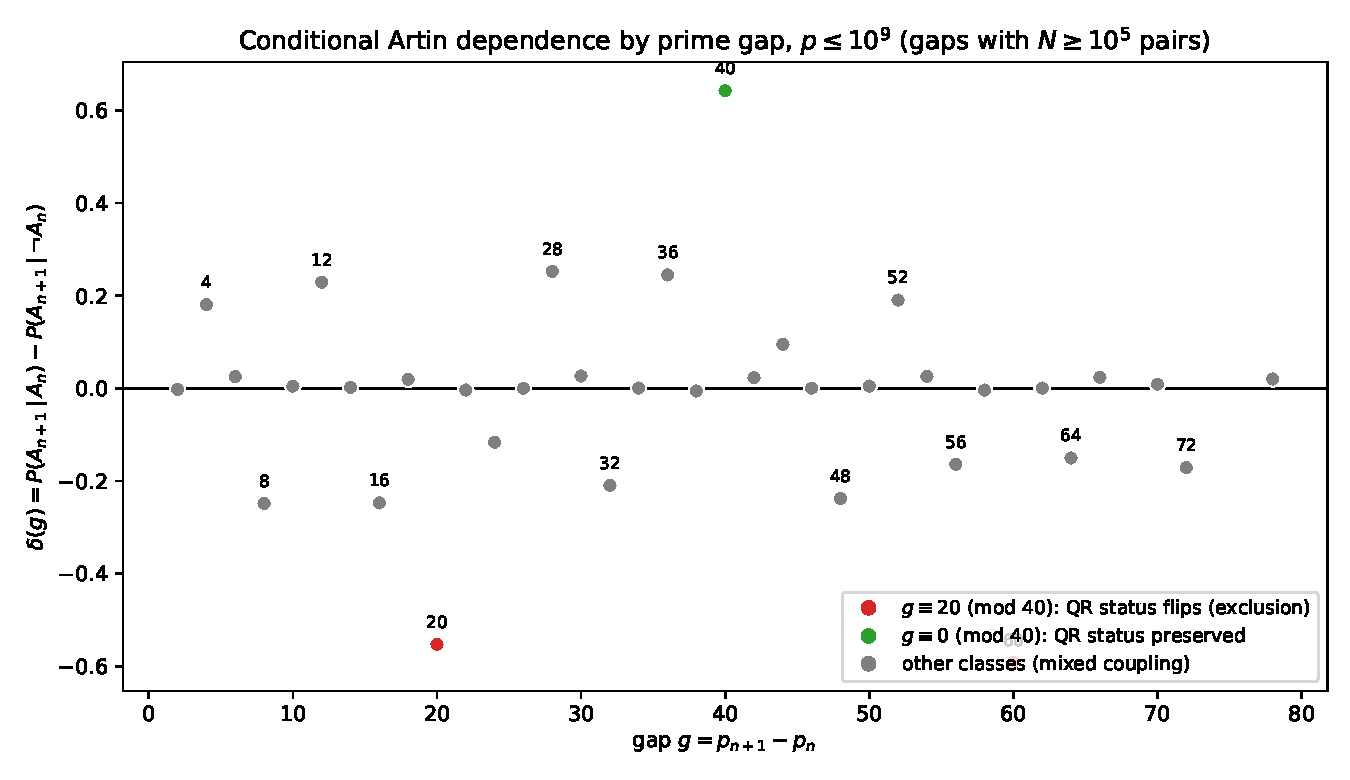
\includegraphics[width=0.95\textwidth]{fig_gap_delta.pdf}
	\caption{$\delta(g)$ for all gaps with $N \ge 10^5$ pairs, $p \le 10^9$. Red:
		$g \equiv 20 \pmod{40}$ (Theorem~\ref{thm:exclusion} forces
		$P(A|A) = 0$). Green: $g \equiv 0 \pmod{40}$
		(Corollary~\ref{cor:coupling} preserves quadratic-residue status). Grey: other
		classes.}
	\label{fig:gaps}
\end{figure}

Three features stand out.

\emph{(i) The exclusion rows.} At $g = 20$ ($1{,}824{,}043$ pairs) and $g = 60$
($371{,}839$ pairs), $P(A \mid A)$ is exactly zero: among $2.2$ million
consecutive pairs, not one is doubly Artin. This is
Theorem~\ref{thm:exclusion} in action, and conversely the observation that
motivated its proof.

\emph{(ii) The $g = 40$ spike.} $P(A \mid A) = 0.899$, the largest conditional
probability in the table and $2.4$ times the unconditional density. Two forced
mechanisms combine. First, by Corollary~\ref{cor:coupling}, if $p_n$ is Artin
then $10$ is a non-residue for $p_{n+1}$ as well, a necessary condition for
the Artin property.
Second, $40 \equiv 1 \pmod 3$ forces the pair's mod-$3$
residues: $p_n \equiv 2 \pmod 3$ would give $3 \mid p_n + 40$, impossible; so
every $g = 40$ pair has $p_n \equiv 1$, $p_{n+1} \equiv 2 \pmod 3$ --- that is,
$3 \mid p_n - 1$ (suppressing $\Art_n$) and $3 \nmid p_{n+1} - 1$ (favouring
$\Art_{n+1}$). Conditioning on $\Art_n$ therefore selects pairs in which
$p_{n+1}$ enjoys both the non-residue status and the mod-$3$ advantage.
These conditions are consistent with the large observed value $0.899$ but do
not quantitatively derive it without an explicit density calculation.

\emph{(iii) Sign classes.} Several gaps that are divisible by $3$ but not
constrained mod~$40$, for instance $6$, $18$, $30$, $42$ and $54$, show a
small positive $\delta \approx +0.02$. A natural guess is that the pair
shares its mod-$3$ status, weakly coupling the largest single suppression
factor. This is a
selected family rather than a rule: other gaps divisible by $3$ and lying in
neither $0$ nor $20$ mod~$40$, such as $12$, $24$ and $36$, do not all
behave this way, and we have no statement covering every class. Some gaps with
adverse mod-$8$ and mod-$5$ shifts show strong negative $\delta$. We can
therefore offer only a qualitative reading of Table~\ref{tab:gaps} in terms of
how the shift by $g$ permutes the residues of $p$ modulo $8$, $5$ and $3$; we
do not derive the entries, and outside the exclusion classes nothing here is
forced.




\section{Residue conditioning}
\label{sec:decomposition}

To what extent does the association persist once the explicit residue channels
are held fixed? We treat what follows as an exploratory conditioning
diagnostic; it does not answer that question quantitatively. We condition on
the \emph{joint} residue class of
$(p_n, p_{n+1})$ to modulus $m$ and measure the residual within-cell
dependence. The statistic reported is the sum of per-cell Pearson $\chi^2$
values over all non-degenerate cells meeting a minimum count threshold,
together with the pair-weighted mean of per-cell~$\delta$. This is a
descriptive aggregate of per-cell associations; it is \emph{not} the standard
Cochran--Mantel--Haenszel statistic (which would be a single one-degree-of-freedom
test of a common association).

Conditioning on $m = 120 = \mathrm{lcm}(8,3,5)$ fixes the quadratic character
$\Lsym{10}{\cdot}$ of both primes (its conductor $40$ divides $120$) and the
mod-$3$ channel. Cells in which $10$ is a quadratic residue for $p_n$ or
$p_{n+1}$ are degenerate for the analysis (one margin of the $2\times2$ table
vanishes --- the Artin property is impossible); the informative population is
roughly a quarter of all pairs, those in doubly-non-residue cells. The
selected populations in Table~\ref{tab:decomp} are the thresholded subsets of
this population: $12{,}255{,}203$ pairs ($24.10\%$ of the census) at
modulus~$120$ and $12{,}086{,}765$ pairs ($23.77\%$) at modulus~$840$. The
unthresholded doubly-non-residue fraction need not be exactly $1/4$.

\begin{table}[ht]
	\centering
	\caption{Selected-cell residual association after conditioning on joint residues
		mod $m$.
		``$\delta_{\mathrm{res}}$'' is the pair-weighted mean within-cell $\delta$
		over non-degenerate cells meeting the count threshold;
		``cells'' is the number of such cells; ``pairs used'' is the total pairs
		in those cells. Cells with fewer than $5000$ ($m = 120$) or $2000$ ($m = 840$)
		pairs are excluded.}
	\label{tab:decomp}
	\begin{tabular}{lrrrr}
		\toprule
		Conditioning           & cells & pairs used     & $\sum \chi^2$ (df) & $\delta_{\mathrm{res}}$ \\
		\midrule
		none (global)          & 1     & 50{,}847{,}530 & 10{,}167 \ (1)     & $-0.014140$             \\
		mod 120 joint residues & 145   & 12{,}255{,}203 & 789.2 \ (145)      & $-0.001055$             \\
		mod 840 joint residues & 633   & 12{,}086{,}765 & 719.8 \ (633)      & $-0.000473$             \\
		\bottomrule
	\end{tabular}
\end{table}

\textbf{Interpretation and limitations.}
The three statistics in Table~\ref{tab:decomp} have successively smaller
absolute values: $-0.0141$ (global) then $-0.00106$ (mod~$120$, $145$~cells
covering $12.3$~million pairs) then $-0.00047$ (mod~$840$, $633$~cells
covering $12.1$~million pairs). We emphasise that these are three different
quantities computed on three different populations, not one quantity being
reduced; the comparison is an exploratory conditioning diagnostic, not a
decomposition. Note also that a signed mean can be small because sizable
positive and negative within-cell associations cancel, so smallness in this
metric is not by itself evidence that dependence has gone. The summed per-cell
$\chi^2$ at mod~$840$ is $719.8$ on $633$ nominal degrees of freedom
($\chi^2/\mathrm{df} = 1.14$); we do not read $\chi^2/\mathrm{df} \approx 1$
as the disappearance of dependence, since no reference distribution has been
established for this serially structured, selected collection.
Two further observations: (i) the three values decrease in magnitude in the
order stated ($-0.0141$, $-0.00106$, $-0.00047$); (ii) a
split-sample check (pairs with $p < 5 \times 10^8$ versus
$p \ge 5 \times 10^8$, conditioning mod $120$) gives residuals
$-0.00096$ and $-0.00094$ --- stable across the range.

Several caveats apply. The global $\delta$ over $50.8$ million pairs and the
selected-cell $\delta_{\mathrm{res}}$ over $12.1$~million selected informative
pairs are \emph{different estimands on different populations}; arithmetic
comparison of their magnitudes is descriptive but does not constitute a proper
decomposition. A marginal risk difference is not, in general, the pair-weighted
mean of stratum risk differences without a between-group term and specified
weights. The per-cell Pearson calibration assumes independent observations
within each cell, which is not established for this serially structured
deterministic census. The paper does not specify a numerical model for the
omitted channels against which ``compatible'' could be formally tested. Those
omitted channels are not only the divisibility channels at $q \ge 11$:
fixing $p$ modulo $840$ determines whether $3$, $5$ and $7$ divide $p - 1$,
but not whether $10^{(p-1)/q} \equiv 1 \pmod p$ when one of them does, so
cubic and higher power-residue obstructions at these same small primes are
also unmodelled. The mod-$3$ channel here is the divisibility channel, not the
full cubic-residue condition.

Joint-residue conditioning yields a smaller selected-cell signed
residual association than the global figure. The remaining association is small in that metric but is
not established to vanish. These results are consistent with a substantial role
for arithmetic residue structure; they do not constitute a complete
decomposition or an independent quantitative verification of the
Hardy--Littlewood-based explanation of the consecutive-prime bias.




\section{The intermediate link: repulsion of \texorpdfstring{$\omega(p-1)$}{omega(p-1)}}
\label{sec:omega}

The chain from residue bias to Artin status passes through the factorisation
of $p - 1$. Its first summary statistic is
$\omega(p-1)$, the number of distinct prime factors, which has normal order
$\log\log p$ over shifted primes $p - 1$ --- a classical result of
Erd\H{o}s~\cite{Erdos1935}. (We invoke the normal order only; we do not use a
mean-value asymptotic, which would need separate tail control.) If consecutive primes repel modulo every small
$q$, then $q \mid p_n - 1$ makes $q \mid p_{n+1} - 1$ \emph{less} likely than
average, and summing over $q$ one predicts a negative correlation between
$\omega(p_n - 1)$ and $\omega(p_{n+1} - 1)$.

The data confirm this with a value that is, to our knowledge, unreported:
\[
	r\bigl(\omega(p_n - 1),\, \omega(p_{n+1} - 1)\bigr) = -0.0410
	\qquad (50{,}847{,}530 \text{ pairs}, \; p \le 10^9).
\]
The factorisations of $p - 1$ for consecutive primes are therefore not
independent. We stress that this measurement establishes dependence, not its
cause. The heuristic above accounts only for the same-$q$ terms: writing
$I_q(p) = \mathbf{1}_{q \mid p-1}$,
\[
  \operatorname{Cov}\bigl(\omega(p_n-1), \omega(p_{n+1}-1)\bigr)
  = \sum_q \operatorname{Cov}\bigl(I_q(p_n), I_q(p_{n+1})\bigr)
  + \sum_{q \ne r} \operatorname{Cov}\bigl(I_q(p_n), I_r(p_{n+1})\bigr),
\]
and the cross terms $q \ne r$ are neither estimated nor signed here. Summing
fixed-modulus predictions over all $q$ up to a growing cutoff would in any case
require uniformity and tail control that we do not supply. Nor is $\omega$ a
sufficient statistic for Artin status: which primes divide $p-1$, and whether
$10$ is a $q$th power residue, both matter. The observed repulsion is
consistent with the same residue-class repulsion that governs the primes, but
we do not establish that it has the same cause. The Pearson coefficient is
reported as a descriptive nominal value.




\section{The cross-base correlation}
\label{sec:measurement}

For each pair write $\phi(a,b)$ for the Pearson correlation of the indicator
variables (the $\phi$ coefficient of the $2\times2$ table). This is an exhaustive census of a fixed
interval for a deliberately chosen finite set of bases, so the coefficients
below are exact and carry no sampling error. We therefore report effect sizes
and their variation with $x$, and avoid the vocabulary of statistical
inference. Where a scale factor is quoted we write
$\sigma_0 = N^{-1/2} \approx 0.00014$ at $N \approx 5.08 \times 10^7$: this is
the standard deviation of $\phi$ under an i.i.d.\ independence benchmark that
does \emph{not} describe these data --- the primes are enumerated, not
sampled --- and ratios $\phi/\sigma_0$ should be read as model-relative
diagnostics indicating that the effects are far larger than that benchmark's
scale, not as tests of any hypothesis. No claim below depends on such a ratio.

One convention should be stated, since it affects the conditional averages in
Sections~\ref{sec:decomposition_crossbase} and~\ref{sec:entanglement}. Within-cell $\phi$
is undefined when a cell is constant in one of the two indicators (for example
cells with $5 \mid p-1$, in which no prime is Artin base $5$). Such cells carry
zero conditional covariance and are omitted from the pooled average, which
therefore draws on $73\%$ of primes on average for the signature
stratification, and $23\%$ for the finer signature-plus-character
stratification, where three of the four character quadrants are identically
non-Artin. Explicitly, for a base pair $(a,b)$ we report
\[
  \phi \mid \mathrm{sig} \;=\;
  \frac{\sum_{s \in E_{ab}} n_s\,\phi_{ab,s}}{\sum_{s \in E_{ab}} n_s},
\]
where $s$ runs over signature cells, $n_s$ is the number of primes in cell $s$,
and $E_{ab}$ is the set of cells with $n_s \ge 200$ in which \emph{both}
indicators vary. This is a prime-count-weighted descriptive mean of within-cell
correlations, not a partial correlation coefficient and not an additive
component of $\phi$; outer means over the $66$ base pairs are unweighted.
Pooling instead on the covariance scale over all cells, which
requires no such exclusion, gives $95.3\%$ removal, in agreement with
Table~\ref{tab:decomp_crossbase}.

\begin{table}[t]
\centering
\caption{Same-prime cross-base Artin correlation at $x = 10^9$: summary and
extremes. ``Triple-completed'' means the base set contains a third base $c$ with
$\sqf(c) = \sqf(ab)$. This is a property of the chosen base set, not of the
pair: the two bases of such a pair are multiplicatively independent in the
usual sense, and adding or removing $c$ changes the label but not the pair's
density, character or Kummer field.}
\label{tab:summary}
\begin{tabular}{lrr}
\toprule
 & pairs & mean $\phi$ \\
\midrule
all pairs & $66$ & $+0.0352$ \\
non-completed & $51$ & $+0.0363$ \\
triple-completed & $15$ & $+0.0314$ \\
\midrule
largest: $(5,13)$ & & $+0.0667$ \\
smallest: $(3,15)$ & & $-0.0303$ \\
second smallest: $(2,10)$ & & $-0.0302$ \\
\bottomrule
\end{tabular}
\end{table}

\begin{table}[t]
\centering
\caption{The ten largest $|\phi|$ at $x = 10^9$, with the values after
conditioning on $\omega(p-1)$ and on the fine signature $\mathrm{sig}(p)$
(pair-weighted mean of within-cell $\phi$; cells with fewer than $200$
primes excluded). ``TC''\ marks triple-completed pairs.}
\label{tab:top}
\begin{tabular}{rrrrrc}
\toprule
$a$ & $b$ & $\phi$ & $\phi \mid \omega$ & $\phi \mid \mathrm{sig}$ & TC \\
\midrule
$5$ & $13$ & $+0.0667$ & $+0.0200$ & $+0.0003$ & \\
$5$ & $17$ & $+0.0649$ & $+0.0218$ & $+0.0025$ & \\
$5$ & $29$ & $+0.0631$ & $+0.0246$ & $+0.0007$ & \\
$5$ & $10$ & $+0.0624$ & $+0.0285$ & $-0.0125$ & \checkmark \\
$5$ & $6$  & $+0.0623$ & $+0.0292$ & $+0.0005$ & \\
$5$ & $11$ & $+0.0623$ & $+0.0300$ & $+0.0004$ & \\
$5$ & $15$ & $+0.0622$ & $+0.0297$ & $-0.0255$ & \checkmark \\
$3$ & $5$  & $+0.0622$ & $+0.0284$ & $+0.0015$ & \checkmark \\
$5$ & $7$  & $+0.0622$ & $+0.0297$ & $+0.0002$ & \\
$2$ & $5$  & $+0.0621$ & $+0.0336$ & $+0.0004$ & \checkmark \\
\bottomrule
\end{tabular}
\end{table}

Three observations, in increasing order of depth.

\begin{observation}[Positivity]
\label{obs:positive}
$\phi(a, b) > 0$ for $64$ of the $66$ pairs. Artin statuses of different
bases at the same prime \emph{attract}.
\end{observation}

The sign is the opposite of the consecutive-prime correlation measured above
(\S\ref{sec:global}, where $\delta < 0$), and the
mechanism is transparent: there the two primes had \emph{different} (and
LOS-anticorrelated) values of $p - 1$; here every base is tested against the
\emph{same} $p - 1$. If $p - 1$ has few small prime factors and a small
$2$-part, the primitive-root condition is easier for every base at once.
Formally, the Artin indicators share the common cause $\mathrm{sig}(p)$.

\begin{observation}[The negative pairs are triple-completed]
\label{obs:negative}
The only pairs with $\phi < 0$ are $(2, 10)$ and $(3, 15)$: in each, the
product of the two bases is, up to a square, the third base of a
multiplicative triple contained in the set ($2 \cdot 10 = 4 \cdot 5$,
$3 \cdot 15 = 9 \cdot 5$). For $(2, 10)$:
$P(\Acal_{10} \mid \Acal_2) = 0.3551$ versus
$P(\Acal_{10} \mid \lnot\Acal_2) = 0.3853$.
\end{observation}

The sign reversal is where Theorem~\ref{thm:pair} becomes visible statistically. For every pair, triple-completed or not, the primes split into two halves according to the sign
of $\chi_d(p)$, $d = \sqf(ab)$: on the half with $\chi_d(p) = -1$ the values
$\chi_a(p)$ and $\chi_b(p)$ are forced \emph{opposite}, so joint Artin status
is impossible there, while on the half with $\chi_d(p) = +1$ they are forced
\emph{equal} and joint Artin status is unobstructed. This is visible directly
in the data: over all $66$ pairs and all $50{,}847{,}524$ primes, the number of
primes Artin for both bases with $\chi_a(p) \ne \chi_b(p)$ is exactly zero,
while the conditional joint density on the complementary half is
$0.299$.

What then distinguishes the two negatively correlated pairs is not the
existence of the exclusion --- every one of the $66$ pairs has it, on exactly
half the primes --- but the identity of the barring character $\chi_d$, and in
particular how its conductor interacts with the common cause $p-1$. Among the
fifteen triple-completed pairs, $d = \sqf(ab)$ takes the values
$\{2, 3, 5, 6, 7, 10, 15, 21\}$, and the two pairs with $d = 5$ ---
$(2,10)$ and $(3,15)$, of conductor $5$, the smallest conductor occurring and
the only odd prime one --- are exactly the two with $\phi < 0$. That is the
sharp empirical discriminant: not dependence, which thirteen positively
correlated pairs also enjoy, but $\mathrm{cond}(\sqf(ab)) = 5$. A plausible
reading is that a small conductor makes the barring condition
$\chi_d(p) = -1$ resolve on a coarse residue class that is comparatively well
correlated with the divisibility structure of $p-1$ driving the common cause,
so the exclusion survives the averaging instead of being diluted by it; we do
not have a proof of this and record it as an observation.
Section~\ref{sec:entanglement} tests the reading by conditioning the common
cause away, after which the exclusion becomes visible on six triple-completed pairs rather than two.




\section{Decomposition: the correlation is the structure of \texorpdfstring{$p-1$}{p-1}}
\label{sec:decomposition_crossbase}

\begin{table}[t]
\centering
\caption{Mean cross-base correlation after conditioning, all $66$ pairs at
$x = 10^9$. ``Removed'' is
$1 - \lvert\overline{\phi_{\mathrm{cond}}}\rvert / \lvert\overline{\phi}\rvert$,
the means taken signed over the $66$ pairs; on the mean-absolute scale the
corresponding figures are $51\%$ and $87\%$, and on the covariance scale
$57\%$ and $95\%$.}
\label{tab:decomp_crossbase}
\begin{tabular}{lrr}
\toprule
conditioning & mean $\phi$ & removed \\
\midrule
none & $0.0352$ & --- \\
$\omega(p-1)$ & $0.0158$ & $55\%$ \\
$\mathrm{sig}(p)$: $\bigl(v_2,\ \{q \le 13\},\ \omega_{>13}\bigr)$
  & $0.0019$ & $95\%$ \\
\bottomrule
\end{tabular}
\end{table}

Conditioning on $\omega(p-1)$ alone --- the crude size of the factorisation
--- removes barely half of the correlation. This is worth emphasising because
$\omega$ is the statistic through which the consecutive-prime papers routed
the mechanism, and it is genuinely insufficient here: two primes with the same
$\omega(p-1)$ can present very different Artin conditions (it matters
\emph{which} primes divide $p-1$, and with what $2$-adic valuation, not how
many). The fine signature --- $2$-adic valuation capped at $4$, the exact set
of primes $\le 13$ dividing $p - 1$, and the count of larger prime factors
capped at $3$ --- is the information the Artin criterion actually consults
for small bases, and conditioning on it removes $95\%$ of the mean
correlation (Table~\ref{tab:decomp_crossbase}). That the fine structure of $p-1$, rather
than its coarse size, is what governs Artin behaviour is in the same spirit as
the refined order-distribution conjectures
of~\cite{GoldmakherMartinPeringuey2025}, which pass from the Artin condition
$\mathrm{ord}_p(a) = p-1$ to the distribution of
$\omega\bigl((p-1)/\mathrm{ord}_p(a)\bigr)$ --- finer information about the
index than its mere vanishing, just as our signature is finer information about
$p-1$ than $\omega(p-1)$.

We regard this as the main statistical finding: \emph{cross-base Artin
correlation at a single prime is, to first order, not an interaction between
the bases at all}. It is a common-cause effect of the shared integer $p - 1$.
A model that reproduces the observed within-signature conditional marginals
and the observed signature frequencies --- equivalently, one in which the two
indicators are conditionally independent given the signature --- accounts for
$95\%$ of the observed mean association. Conditional independence alone is not
enough: an independent model with constant cell probabilities is an immediate
counterexample.




\section{The residual and the exclusion law}
\label{sec:entanglement}

The $5\%$ that survives is not uniformly distributed: it is concentrated on the triple-completed pairs. This section argues that it is the statistical trace of Theorem~\ref{thm:pair} --- the
deterministic exclusion that the unconditional correlation of
Section~\ref{sec:measurement} had largely averaged away.

\begin{table}[t]
\centering
\caption{Residual correlation after conditioning on $\mathrm{sig}(p)$ and
after additionally conditioning on the pair of quadratic-residue statuses
$(\chi_a(p), \chi_b(p))$, split by triple-completion. All values at
$x = 10^9$ over $50{,}847{,}524$ primes.}
\label{tab:residual}
\begin{tabular}{lrrr}
\toprule
group & mean $\phi$ & mean $\phi \mid \mathrm{sig}$
      & mean $\phi \mid \mathrm{sig}, \mathrm{QR}$ \\
\midrule
triple-completed ($15$ pairs)   & $+0.0314$ & $+0.0049$ & $+0.0049$ \\
\quad mean \emph{absolute} residual        &           & $\;\;0.0179$ & \\
non-completed ($51$ pairs) & $+0.0363$ & $+0.0010$ & $+0.0052$ \\
\quad mean \emph{absolute} residual        &           & $\;\;0.0010$ & \\
\midrule
all $66$ pairs                            & $+0.0352$ & $+0.0019$ & $+0.0052$ \\
\bottomrule
\end{tabular}
\end{table}

Two facts pin down the mechanism, both measured over the full $10^9$ range.

First, after fine conditioning the triple-completed pairs retain substantial residuals, and every pair with a substantial \emph{negative} residual is
triple-completed. The six pairs below are the only ones with
$\phi \mid \mathrm{sig} < -0.004$, and all six are triple-completed. We state this as
the exact combinatorial fact it is --- six of the six most negative residuals fall in the triple-completed class --- rather than attaching a $p$-value to it: the
$66$ pairs share endpoints and the base set was chosen to contain
multiplicative triples, so the pair labels are neither independent nor
exchangeable and no randomisation model licences such a test.
\[
  \begin{aligned}
    (2,10)&\!:\, -0.0343, &\quad (5,15)&\!:\, -0.0255, &\quad (6,10)&\!:\, -0.0144, \\
    (5,10)&\!:\, -0.0125, &\quad (7,21)&\!:\, -0.0060, &\quad (10,15)&\!:\, -0.0049 .
  \end{aligned}
\]
At $x = 10^9$ these are also the only six negative residuals of any size, but
that sharper statement is not stable with $x$: at $x = 3 \times 10^7$ a further twelve pairs have residuals marginally below
zero, all within $3\sigma_0$ of it in the benchmark scale of
Section~\ref{sec:measurement}.

The residual is not sign-definite, and we record the exceptions explicitly.
Nine of the fifteen triple-completed pairs have \emph{positive} residuals: eight of
them small, and one, $(2,6)$, a large outlier at $+0.1598$ --- the largest
residual of any pair in the collection. Its mechanism is transparent and is the same
entanglement phenomenon seen from the other side: $\sqf(6) = 2 \cdot 3$. The relevant family is narrower than $3 \nmid p-1$ alone, however. If $3 \nmid p-1$ and $v_2(p-1) \ge 2$ then $p \equiv 5 \pmod{12}$, so $(3/p) = -1$ and Theorem~\ref{thm:pair} \emph{forbids} $2$ and $6$ together. Agreement can occur only on the complementary family $v_2(p-1) = 1$, that is $p \equiv 11 \pmod{12}$, where $(3/p) = +1$ and the two quadratic characters coincide; that the remaining odd-prime tests then also very nearly coincide is what we measure, not something the factorisation $\sqf(6) = 2 \cdot 3$ implies on its own, and the signature records whether $3 \mid p-1$ without recording the
resulting near-determinism inside those cells. (The effect is sharpest in the cells where $p-1$ has no small odd prime factor
at all: for $v_2(p-1) = 1$, no prime $q \le 13$ dividing $p-1$ and exactly one
larger factor, the $2 \times 2$ table for $(2,6)$ is exactly diagonal over
$1{,}775{,}686$ primes, giving $\phi = +1$. Across the $47$ cells with
$v_2(p-1) = 1$, $3 \nmid p-1$ and at least $200$ primes, the within-cell $\phi$
ranges from $+0.39$ to $+0.98$, so the near-determinism is a feature of that family of cells rather
than of a single one.) The triple-completed-group mean absolute residual of $0.0179$ is
substantially driven by this one pair: excluding it, the figure is $0.0077$,
still eightfold the value for the remaining pairs of $0.0010$. Conditioning
additionally on $(\chi_a(p), \chi_b(p))$ reduces $(2,6)$ to $+0.0055$, in line
with every other pair --- so the outlier is explained by the entanglement
account rather than in tension with it.
Note that $(2,10)$ and $(5,15)$ are more negative \emph{after} conditioning
than before, and that $(5,10)$, $(5,15)$, $(6,10)$, $(10,15)$ and $(7,21)$
change sign under conditioning: the common-cause channel had been masking an
underlying repulsion.

Second, additionally conditioning on the pair of quadratic-residue statuses $(\chi_a(p), \chi_b(p))$ removes the negative residuals. We put it this way deliberately: the signed group means do not both fall to zero. The triple-completed mean stays at $+0.0049$ while the mean for the remaining pairs \emph{rises} from $+0.0010$ to $+0.0052$, and the two averages are taken over different eligible populations (about $73\%$ of primes for signature conditioning against $23\%$ here), so they are not components of a single decomposition. Every one of the
six negative values above becomes positive and small
($+0.0031$, $+0.0066$, $+0.0045$, $+0.0065$, $+0.0040$, $+0.0048$
respectively), and the triple-completed and remaining groups become indistinguishable at $+0.0049$ and $+0.0052$ (Table~\ref{tab:residual}).
That common small positive floor of about $+0.005$ is present for all $66$
pairs and is plausibly attributable to residual odd-prime conditions shared through $p-1$ beyond what our signature records. We note that a \emph{quartic} channel is not available as an explanation here: a fourth power is a square, and in the only quadrant contributing defined correlations both bases are quadratic nonresidues, so no further $2$-power residue condition can bind.

Conditioning on the quadratic characters is precisely what removes
character-level entanglement, and that it flattens the triple-completed pairs is consistent with the residual as the statistical trace of the relation
$\chi_a \chi_b = \chi_{\sqf(ab)}$ --- the same object that makes
Theorem~\ref{thm:pair} true.

One part of this can be made exact, though it is a statement about support and not about the residual's size.
Theorem~\ref{thm:pair} asserts that the joint Artin event is empty on the
stratum $\chi_a(p) \ne \chi_b(p)$, and this is what the contingency tables
show: summing the joint-Artin cell over all signature classes and all $66$
pairs, the count of primes $p \le 10^9$ that are Artin for both $a$ and $b$
with $\chi_a(p) \ne \chi_b(p)$ is
\[
  0 \qquad \text{(out of } 50{,}847{,}524 \text{ primes, for every one of the
  } 66 \text{ pairs)},
\]
while on the complementary stratum the joint density is $0.299$. The support restriction is therefore a theorem rather than a conjecture. It does not by itself determine the sign or the magnitude of any residual: a support constraint of this kind is compatible with zero covariance, as the trivial example of two independent fair signs with Artin indicators given by their negative-sign indicators shows. What the residual measures is a quadratic-information component; that this component is the pointwise law's statistical trace is an interpretation the data support, not a consequence of the theorem.

One caveat on the strength of the flattening step, in the other direction.
Within a $(\chi_a, \chi_b)$ stratum the exclusion cannot operate at all: by
criterion~\eqref{eq:obstruction} an Artin prime for $a$ has $\chi_a(p) = -1$, so all the \emph{joint} Artin mass sits in the single quadrant $(-1,-1)$. In each of the other three quadrants at least one of the two indicators is identically zero, so the within-cell correlation is undefined and the conditional covariance vanishes; this is not the same as saying neither indicator varies there. Conditioning on
$(\chi_a, \chi_b)$ therefore \emph{restricts attention to the stratum on which
the constraint of Theorem~\ref{thm:pair} is vacuous}, and the vanishing of the
residual there is in part a structural consequence of that restriction rather
than an independent confirmation. What the step establishes is the
localisation: the residual lives in the character channel and not elsewhere in
the signature. We state it in that weaker form.

The picture that emerges is cleanly layered:
\[
  \underbrace{\text{common cause } p-1}_{\approx 95\%}
  \;+\;
  \underbrace{\text{quadratic entanglement } \chi_a\chi_b = \chi_{\sqf(ab)}}_{\text{residual, localised on triple-completed pairs}}
  \;+\;
  \underbrace{\text{higher-order sharing}}_{\text{small positive floor}}.
\]




\section{Comparison with the predicted joint densities}
\label{sec:model}

The measurements of Sections~\ref{sec:measurement}--\ref{sec:entanglement}
identify the mechanisms empirically. We now check them against theory
quantitatively, by computing the joint densities predicted by the
Matthews--Moree--Stevenhagen framework and comparing with the observed counts pair by
pair.

Write $d_a = \sqf(a)$. The heuristic, in the form originating
with~\cite{Matthews1976} and systematised by the character-sum method
of~\cite{MoreeStevenhagen2014} (with the general framework
in~\cite{JarviniemiPeruccaSgobba2025}), is an inclusion--exclusion over the
degrees of the Kummer extensions that detect the conditions ``$a$ is an
$\ell$-th power residue'':
\begin{equation}
\label{eq:model}
  \mathbf{P}\bigl(p \in \Acal_a \cap \Acal_b\bigr)
  \;=\; \sum_{m, n \text{ squarefree}}
  \frac{\mu(m)\,\mu(n)}
       {\bigl[\Q(\zeta_L, a^{1/m}, b^{1/n}) : \Q\bigr]},
  \qquad L = \mathrm{lcm}(m,n),
\end{equation}
and the entanglement enters through the degree in the denominator. Generically
\[
  [\Q(\zeta_L, a^{1/m}, b^{1/n}):\Q] = \varphi(L)\,m\,n ,
\]
but the degree drops by the order of the subgroup of quadratic classes
realised inside $\Q(\zeta_L)$, taken from the group
\[
  V(m,n) = \bigl\langle\, d_a \text{ (if $2 \mid m$)},\;
                          d_b \text{ (if $2 \mid n$)} \,\bigr\rangle
  \subseteq \Q^\times/(\Q^\times)^2
\]
whose quadratic field lies inside $\Q(\zeta_L)$, i.e.\ whose conductor divides
$L$. The point of contact with Theorem~\ref{thm:pair} is that when both
$2 \mid m$ and $2 \mid n$ the group $V$ contains not only $d_a$ and $d_b$ but
their product $d_a d_b \sim \sqf(ab)$, so the barring character
$\chi_{\sqf(ab)}$ of Theorem~\ref{thm:pair} is present in the model as a
potential source of degree collapse. Two things must be said precisely here,
because a natural stronger reading is false. First, the product class lies in
$V(m,n)$ for \emph{every} pair of bases whenever both indices are even; its
membership is automatic and has nothing to do with whether a third base of our
set completes a multiplicative triple. Second, membership in $V$ is not
collapse: a class contributes only when its conductor divides $L$. These two
conditions do not coincide, in either direction. For $(7,11)$ --- a pair
outside every triple of our set --- the product class $77$ has conductor $77$,
which divides $L = 154$, while the individual conductors $28$ and $44$ do not,
so the product class does contribute a collapse there. Conversely for $(2,6)$
--- a pair inside the triple $(2,3,6)$ --- the nontrivial classes of $V$ have
conductors $8$, $24$ and $12$, all divisible by $4$, and no squarefree $L$ is,
so no term of~\eqref{eq:model} receives this correction at all. The
triple-completion classification used in our tables is therefore a property of
the chosen base set, not a field-theoretic invariant of the pair, and it is not
equivalent to the occurrence of an extra degree collapse. We evaluate~\eqref{eq:model}
by summing the ramified part exactly over all squarefree $m, n$ supported on
$S = \{2\} \cup \{q : q \mid d_a d_b\}$ and folding the rest into the Euler
product $\prod_{q \notin S}\bigl(1 - \tfrac{2q-1}{q^2(q-1)}\bigr)$,
truncated at $3 \times 10^6$.

As a check on the implementation, the same code specialised to a single base
reproduces the classical Hooley densities: $0.373956$ for bases with
$d \not\equiv 1 \pmod 4$ (Artin's constant), $0.393638$ for $d = 5$,
$0.376368$ for $d = 13$, against measured $0.373957$, $0.393642$, $0.376362$.

\begin{table}[t]
\centering
\caption{Predicted versus measured joint Artin densities, selected pairs at
$x = 10^9$. ``TC''\ marks triple-completed pairs. The final two rows are the two negatively correlated pairs.}
\label{tab:model}
\begin{tabular}{rrrrrrrc}
\toprule
$a$ & $b$ & measured $j$ & model $j$ & rel.\ err.
    & measured $\phi$ & model $\phi$ & TC \\
\midrule
$5$  & $13$ & $0.163939$ & $0.163943$ & $+0.00\%$ & $+0.0667$ & $+0.0667$ & \\
$5$  & $10$ & $0.161962$ & $0.161922$ & $-0.02\%$ & $+0.0624$ & $+0.0623$ & \checkmark \\
$5$  & $15$ & $0.161934$ & $0.161922$ & $-0.01\%$ & $+0.0622$ & $+0.0623$ & \checkmark \\
$3$  & $7$  & $0.149965$ & $0.149971$ & $+0.00\%$ & $+0.0432$ & $+0.0433$ & \checkmark \\
$13$ & $17$ & $0.150249$ & $0.150261$ & $+0.01\%$ & $+0.0383$ & $+0.0383$ & \\
$2$  & $3$  & $0.147361$ & $0.147349$ & $-0.01\%$ & $+0.0321$ & $+0.0321$ & \checkmark \\
$2$  & $6$  & $0.147334$ & $0.147349$ & $+0.01\%$ & $+0.0320$ & $+0.0321$ & \checkmark \\
$7$  & $21$ & $0.144754$ & $0.144728$ & $-0.02\%$ & $+0.0238$ & $+0.0238$ & \checkmark \\
$15$ & $21$ & $0.144725$ & $0.144728$ & $+0.00\%$ & $+0.0237$ & $+0.0238$ & \\
\midrule
$3$  & $15$ & $0.132769$ & $0.132776$ & $+0.01\%$ & $-0.0303$ & $-0.0302$ & \checkmark \\
$2$  & $10$ & $0.132776$ & $0.132776$ & $+0.00\%$ & $-0.0302$ & $-0.0302$ & \checkmark \\
\bottomrule
\end{tabular}
\end{table}

\begin{observation}[The model reproduces the measurements]
\label{obs:model}
Over all $66$ pairs at $x = 10^9$, the mean absolute relative error between
the predicted and measured joint densities is $0.012\%$, with maximum
$0.040\%$ (attained at $(21,29)$). In particular the model predicts the sign reversal: for the negatively correlated pairs $(2,10)$ and $(3,15)$ it gives
$j = 0.132776$ and $\phi = -0.0302$ for both, against measured
$j = 0.132776$, $0.132769$ and $\phi = -0.0302$, $-0.0303$ respectively.
\end{observation}

This is the quantitative counterpart of Sections~\ref{sec:measurement} and~\ref{sec:entanglement}. It is a comparison of unconditional joint densities, so it does not by itself validate any conditional mechanism, but it is a demanding test and the framework passes it. The
$66$-pair pattern --- positive correlation almost everywhere, negative precisely on the two pairs where it is observed to be negative, with magnitudes ordered as observed
--- is not merely \emph{consistent with} the Matthews--Moree--Stevenhagen framework; it is
reproduced by it to within a few parts in $10^4$, with no fitted parameters.
Correspondingly, the same quadratic class $\sqf(ab)$ governs the deterministic law of Theorem~\ref{thm:pair} and enters the heuristic through the group $V(m,n)$. We stop short of calling these one object: the class lies in $V(m,n)$ for every pair once both indices are even, while it lowers a degree only when its conductor divides $L$, and the two conditions come apart in both directions as noted in Section~\ref{sec:model}.

\begin{remark}
\label{rem:eps}
The residual discrepancies are uniformly small (all $66$ pairs below
$0.040\%$) and we have not pursued them; ordinary Hooley-type errors of this
size are expected at $x = 10^9$, since the convergence in Hooley's theorem is
only logarithmic, and our Euler products are truncated at $3 \times 10^6$.
We record one methodological warning, since it cost us a draft. Computing
$\varepsilon(m,n)$ as $2$ raised to the number of classes of $V(m,n)$ with
conductor dividing $L$ --- rather than as the order of the subgroup of $V(m,n)$
realised in $\Q(\zeta_L)$ --- inflates $\varepsilon$ to $8$ on exactly those
pairs with $d_a \equiv d_b \equiv 1 \pmod 4$, where all three of
$d_a, d_b, \sqf(ab)$ have odd conductor. Since $V(m,n)$ has two generators,
$|V(m,n)| \le 4$ and $\varepsilon = 8$ is impossible. The error is invisible in
the single-base specialisation, which is why the check above does not catch it;
it inflates the mean relative error over the $66$ pairs from $0.012\%$ to
$0.037\%$ and concentrates the damage on the ten pairs drawn from
$\{5, 13, 17, 21, 29\}$.
\end{remark}




%% ===================== NEW SECTION: computational content =====================
\section{Computational content: a measured negative}
\label{sec:content}

The correlations above are large by the usual descriptive measures: $\delta = -0.01414$ with a
Pearson statistic of $10{,}167$ on one degree of freedom, and individual cross-base values of
$\phi/\sigma_0$ up to $476$. Those statistics are descriptive, not calibrated: they describe
$5 \times 10^7$ enumerated primes rather than a large effect. The question of this section is
whether the correlation is \emph{computationally} worth anything --- could it predict generator
availability, or yield a faster algorithm? We answer by measurement, for the estimators and the
search workload described below, and within that scope we find no computational use for it. We
record it because the negative is informative and because the protocol transfers to any claimed
predictive advantage in this area.

\subsection*{The right baseline, and two different quantities}
A correlation can look large against a naive reference and carry no usable information once the
elementary structure is taken into account. For consecutive primes that structure is the
\emph{joint residue pair}: a practitioner asking whether $a$ is a primitive root mod $p$ already
knows $p \bmod 4\,\sqf(a)$, and the Legendre symbol $\Lsym{a}{p}$ is a function of it. The correct
baseline for a predictive claim is therefore not the marginal density of $\Art$ but the
conditional distribution given the joint residues.

Two quantities must be distinguished, and earlier drafts of this work conflated them.

\begin{itemize}
	\item An \emph{empirical conditional-entropy diagnostic}: estimate each cell's conditional
	probability from the data and score those same data. This measures how much of the
	variation the conditioning explains, and it is a legitimate descriptive summary --- but a
	finer nested model can never do worse, so it is \emph{not} evidence of predictive skill.
	\item A \emph{held-out} measurement: fit the cell probabilities on one part of the data and
	score a disjoint part. Only this can show predictive value.
\end{itemize}

Table~\ref{tab:content} gives the first quantity on all $50{,}847{,}530$ consecutive pairs below
$10^9$, and Table~\ref{tab:holdout} the second.

\begin{table}[t]
	\centering
	\begin{tabular}{lccc}
		\toprule
		conditioning & entropy (nats) & gain vs marginal & incremental \\
		\midrule
		marginal & $0.661047$ & --- & --- \\
		joint residues mod $120$ & $0.241529$ & $0.419517$ \ ($0.605$ bits) & --- \\
		\quad $+$ predecessor Artin status & $0.241520$ & --- & $\mathbf{0.000009}$ \\
		\midrule
		joint residues mod $840$ & $0.237235$ & $0.423812$ & --- \\
		\quad $+$ predecessor Artin status & $0.237217$ & --- & $\mathbf{0.000018}$ \\
		\bottomrule
	\end{tabular}
	\caption{\emph{Empirical conditional-entropy diagnostic} over $50{,}847{,}530$ pairs below
	$10^9$ (resubstitution: each cell's probability is estimated from the same pairs it scores).
	The elementary joint-residue baseline carries $0.42$ nats; the correlation adds of order
	$10^{-5}$ nats \emph{in this descriptive sense}. This is not a held-out measurement.}
	\label{tab:content}
\end{table}

\begin{table}[t]
	\centering
	\begin{tabular}{llcc}
		\toprule
		baseline & estimator & gain, even$\to$odd & gain, odd$\to$even \\
		\midrule
		joint residues mod $120$ & A & $-3.2\times10^{-6}$ & $-4.9\times10^{-6}$ \\
		& B & $+1.9\times10^{-6}$ & $+9.4\times10^{-8}$ \\
		\midrule
		joint residues mod $840$ & A & $-6.11\times10^{-5}$ & $-6.08\times10^{-5}$ \\
		& B & $-2.55\times10^{-5}$ & $-2.71\times10^{-5}$ \\
		\bottomrule
	\end{tabular}
	\caption{\emph{Held-out} gain, in nats per test pair, from adding the predecessor's Artin
	status to the joint-residue cells. Even$\to$odd: probabilities are fitted on the pairs whose
	successor prime has least significant hash bit $0$ and scored on the complementary half
	($25{,}421{,}106$ pairs); odd$\to$even is the reverse ($25{,}426{,}424$ pairs). Jeffreys
	($+\tfrac12$) smoothing is applied in every cell. Estimator~A splits every cell on the
	predecessor's status; estimator~B does not split a cell whose successor status is constant in
	the fit half, where splitting can only add smoothing penalty. A hash split is used rather than
	a range split because the Artin density drifts with $x$. At modulus $120$ the sign depends on
	the estimator; at modulus $840$ both estimators lose.}
	\label{tab:holdout}
\end{table}

\subsection*{What the in-sample increment is made of}
The in-sample increment of Table~\ref{tab:content} is $0.000009$ nats at modulus $120$ and
$0.000018$ nats at modulus $840$. For scale only: with no association and regular i.i.d.\
sampling, its expectation is $k/(2N)$, where $k$ counts the cells in which both the
predecessor's and the successor's status vary ($k=256$ and $k=1{,}599$), that is
$2.5\times10^{-6}$ and $1.6\times10^{-5}$ nats. That reference is heuristic --- the cells are
sparse and consecutive pairs overlap --- so we calibrate by simulation instead.

The simulation is a \emph{residue-status null}. Every prime's Artin status is redrawn
independently, with probability equal to the observed Artin rate of its residue class modulo
$M$, and the census tables are rebuilt from the simulated statuses. Statuses are drawn per
prime, so each simulated pair is still (status of $p_n$, status of $p_{n+1}$) and the overlap
between consecutive pairs is preserved; by construction the predecessor's status carries no
information beyond residues modulo $M$. Over $100$ replicates for each $M$:
\begin{itemize}
	\item with $M=120$ the null reproduces the reference scale (mean $2.53\times10^{-6}$, standard
	deviation $2.1\times10^{-7}$, for the mod-$120$ increment), and no replicate reaches the
	observed $9.18\times10^{-6}$;
	\item with $M=840$ the null gives a mod-$120$ increment of mean $8.82\times10^{-6}$ (standard
	deviation $4.9\times10^{-7}$), and $24$ of the $100$ replicates reach or exceed the observed value.
\end{itemize}
The excess over the mod-$120$ baseline is therefore residue information: a model in which
statuses depend on nothing but $p \bmod 840$ reproduces it. The residue channel involved is the
prime $7$ of $p-1$, which the mod-$120$ cells do not see: primes $p\equiv 1 \pmod 7$ are Artin
base $10$ at rate $0.3284$, against $0.3831$ for the other classes (ratio $0.857$, consistent with
the heuristic factor $6/7$ for that channel). At modulus $120$ estimator~B of
Table~\ref{tab:holdout} gains slightly ($+1.9\times10^{-6}$ and $+9.4\times10^{-8}$). We have not
tested that held-out figure against the residue-status null, and in view of the in-sample result
we do not treat it as evidence of information specific to the predecessor's status.

Against the mod-$840$ baseline the observed increment, $1.83\times10^{-5}$, lies slightly above
the $M=840$ null (mean $1.71\times10^{-5}$, standard deviation $6.8\times10^{-7}$; $2$ of the $100$
replicates reach it). We do not read this either way: the null is a simulation benchmark with its
own assumption (independent statuses given the residue class), $100$ replicates resolve tail
frequencies only coarsely, and neither held-out estimator gains at modulus $840$.

Within the estimators above, then, the predecessor's Artin status shows no predictive value beyond
the joint residues modulo $840$, and its apparent value beyond residues modulo $120$ is residue
information. We state this as a model- and workload-limited finding, not as an
information-theoretic bound: nothing here bounds the oracle conditional mutual information, other
estimators or other ranges. The same trap appears one level coarser, and a reader who repeats this
should expect it: conditioning on the gap class $g \bmod 40$ \emph{alone} produces a spurious
apparent gain of about $0.02$ nats, because $g \bmod 40$ does not determine the individual
residues $p_n \bmod 40$ and $p_{n+1} \bmod 40$; the apparent signal is residue information
re-appearing. The joint residues, at a modulus that includes every small channel of $p-1$ in
play, are the correct baseline.

\subsection*{What the between-cell share measures}
The global anticorrelation admits an exact two-term decomposition. Writing $X,Y$ for the
predecessor's and successor's Artin indicators and $C$ for the joint-residue cell, the law of
total covariance gives
\[
\delta \;=\; \underbrace{\frac{1}{\operatorname{Var}(X)}\sum_c \pi_c\, r_c(1-r_c)\,\delta_c}_{\text{within}}
      \;+\; \underbrace{\sum_c \bigl(w_c^{1}-w_c^{0}\bigr) p_c}_{\text{between}},
\]
with $\pi_c = P(C{=}c)$, $r_c = P(X{=}1\mid C{=}c)$, $w_c^{x}=P(C{=}c\mid X{=}x)$,
$p_c=P(Y{=}1\mid C{=}c)$ and $\delta_c$ the within-cell association. This is an identity, not a
model. In a cell where the predecessor's status never varies $\delta_c$ is undefined; under this
and every convention below such a cell contributes zero within-cell association (equivalently,
the missing conditional probability is completed by the observed one). The driver accumulates
each within and each between sum independently and asserts the identities; at $10^9$ they hold
to machine precision. The covariance form places $98.69\%$ (mod $120$) and $99.55\%$ (mod $840$)
of $\delta$ between joint-residue cells, with within-cell terms $-0.000186$ and $-0.000064$.

The share depends on the weighting convention. With the Kitagawa ordering and
$P(C{=}c\mid X{=}1)$ weights, whose between term is
$\sum_c (w_c^1-w_c^0)\,P(Y{=}1\mid X{=}0, C{=}c)$, it is $96.14\%$ (mod $120$) and $97.81\%$
(mod $840$); with $P(C{=}c\mid X{=}0)$ weights it is $99.22\%$ and $99.71\%$; with symmetric
weights $97.68\%$ and $98.76\%$. Across these four conventions the between share lies between
$96.1\%$ and $99.2\%$ at modulus $120$, and between $97.8\%$ and $99.7\%$ at modulus $840$.
Cells in which the predecessor's status never varies hold about half of all pairs (a fraction
$0.49996$ at modulus $120$, all of them cells with no Artin predecessor), and by the convention
just stated they contribute only to the between term.

\subsection*{Both exclusion laws are computationally redundant}
An exclusion law can be mathematically correct and computationally useless, and both of ours are
instances of that. The gap law (Theorem~\ref{thm:exclusion}) is the statement that for
$g \equiv 20 \pmod{40}$ the product $\chi_{10}(p)\chi_{10}(p+g)$ is the constant $\mathbf{-1}$
(equivalently $\chi_{10}\bigl(p(p+g)\bigr) = -1$), so the two characters are opposite and at most
one of the two primes can be Artin. The constant sign follows from quadratic reciprocity applied
to the shift $g$, together with multiplicativity; multiplicativity alone does not fix which sign
the shifted product takes. But a practitioner need not track predecessor status or gap state to
learn this: reading $p \bmod 40$ gives $\chi_{10}(p)$ directly, and $p+g \bmod 40$ gives
$\chi_{10}(p+g)$. The law is a statement about characters that a character computation already
answers.

The same is true of the same-prime law (Theorem~\ref{thm:pair}) and its triple corollary
(Theorem~\ref{thm:triple}): they follow from $\chi_c = \chi_a\chi_b$, so if $a$ and $b$ are Artin
then both characters are $-1$ and $\chi_c = +1$, whence $c$ is not Artin whenever the three bases are units modulo $p$
(i.e.\ $p\nmid abc$). To be precise about the scope of ``redundant'': \emph{once the relevant individual
quadratic characters are already available}, these statements supply no further rejection beyond
what those characters give. Both deductions combine characters that are already in hand; for
the gap law, reciprocity is what makes the $\chi_5$ character available in the first place.
Neither saves a
modular exponentiation that a character-aware implementation was not already saving. We verified
the gap law exhaustively at $10^9$ --- $2{,}214{,}511$ pairs with $g \equiv 20 \pmod{40}$, of
which $984{,}678$ have an Artin predecessor, and \emph{zero} are doubly-Artin --- but exhaustive
verification of a redundancy is still a redundancy.

\subsection*{The one usable filter is elementary}
The only filter that does real work is the necessary condition of \S\ref{sec:prelim}: a primitive
root must be a quadratic non-residue, so $\Lsym{a}{p}=-1$. It is answerable in $O(1)$ arithmetic
by reciprocity rather than by exponentiation, and it is exactly the information that the
conductor-$40$ quadratic channel of \S\ref{sec:decomposition} carries. That is the honest reading
of the decomposition: the paper \emph{explains} why a standard filter works, and identifies which
channel carries the effect, but it does not supply a new one.

We measured it in a scanning search for Artin-base-$10$ primes at $p \approx 10^{15}$, where
factorising $p-1$ dominates. The three strategies below are single-threaded loops on a 32-core
machine; the recorded times are kernel times for the search loop itself, with the shared
small-prime setup (identical for all three, and amortised in any real deployment) excluded.

\begin{table}[t]
	\centering
	\begin{tabular}{lccc}
		\toprule
		strategy & time (s) & factorizations of $p-1$ & ratio to naive \\
		\midrule
		naive (factor every prime) & $0.1642$ & $722$ & $1.00\times$ \\
		non-residue filter first & $0.0841$ & $376$ & $1.95\times$ \\
		\quad $+$ small-$\ell$ early exit & $0.0732$ & $300$ & $2.24\times$ \\
		\bottomrule
	\end{tabular}
	\caption{Finding $300$ Artin-base-$10$ primes above $10^{15}$; $722$ primes visited. The
	small-$\ell$ early exit tests the channels $\ell \in \{3,5,7,11,13,17,19\}$ of $p-1$ before
	the full factorisation, rejecting on first failure ($402$ cheap exponentiations). The last
	step is about $15\%$ faster, equivalently about $13\%$ less elapsed time, than the
	non-residue filter alone; the exact counters (primes, factorizations, exponentiations)
	reproduce independently, while timings are single-run and hardware-dependent.}
	\label{tab:filter}
\end{table}

Ordering the small prime channels of $p-1$ before the full factorisation --- testing
$a^{(p-1)/\ell} \not\equiv 1$ for small $\ell \mid p-1$ and rejecting on the first failure ---
saves $20\%$ of the factorizations. This is a \emph{test-ordering} principle rather than a new
algorithm, and it is workload-dependent in a way worth stating: if the task is to find \emph{any}
primitive root for a \emph{given} $p$, then $p-1$ is factored once and cached, and the early exit
saves the cheap exponentiations but not the factorisation at all. The gain exists only for
scanning searches over fresh primes.

\subsection*{What would change the verdict}
This is a negative assessment of the evidence, not an impossibility theorem. The conditioning
above does not prove exact conditional independence, and the verdict would change if: (i)~a
repeated workload existed in which many compatible primes or candidate bases are tested and the
required labels are already available; (ii)~a new \emph{deterministic} exclusion were found that
rules out a case the character deductions do not already rule out; (iii)~an actionable decision
followed from the correlation --- skipping a soundly excluded candidate, or reordering costly
tests --- with net cost falling after factorisation, feature acquisition and bookkeeping; and
(iv)~correctness were preserved, since a predictor may order tests but cannot replace
certification. None of these holds in the workloads tested here. We have not evaluated a
cross-base predictive workload at all, so the negative is demonstrated for the consecutive-prime
axis and for the scanning-search workload; the same-prime axis is covered only by the redundancy
argument above. The results are best understood as describing arithmetic structure, and as
identifying exactly which elementary structure the observed correlations are made of.



%% ===================== MERGED DISCUSSION + DECLARATIONS =====================
\section{Discussion}
\label{sec:discussion}

\subsection*{What is new here}
The individual ingredients are classical: quadratic reciprocity, the quadratic-residue
obstruction to primitive roots, the consecutive-prime bias of~\cite{LOS2016}, and the
Kummer-degree density computations of~\cite{Matthews1976,MoreeStevenhagen2014}. The
contributions of this paper are: (i)~the observation that these combine into deterministic
exclusion laws on both axes --- a gap law for consecutive primes at base $10$
(Theorem~\ref{thm:exclusion}) and a same-prime pair law with a triple corollary
(Theorem~\ref{thm:pair}, Theorem~\ref{thm:triple}). The gap law is the base-$10$ instance of
the phenomenon identified by Tinkov\'a--Waxman--Zindulka~\cite{TinkovaWaxmanZindulka2023},
and we claim no priority for it; (ii)~a measurement, at the scale of $10^9$ primes, of the
consecutive-prime Artin correlation, its gap profile, and the $\omega$ repulsion, together
with the cross-base correlations $\phi(a,b)$ and their joint-density comparison; (iii)~a
descriptive reduction showing that, depending on the weighting convention, $96.1$--$99.2\%$
(modulus $120$) and $97.8$--$99.7\%$ (modulus $840$) of the consecutive-prime anticorrelation
lies between joint-residue cells, and that $95\%$ of the mean
cross-base correlation is removed by conditioning on the fine signature of $p-1$ --- that is,
both correlations are largely accounted for by the same elementary structure
--- the residues of $p$ and the factorisation of $p-1$ --- rather than by an interaction
(reductions of different estimands on different selected populations, not a complete
decomposition); and (iv)~a measured audit of the computational content
of those correlations, which finds no computational use for them within the estimators and the
workload tested (\S\ref{sec:content}). The exclusion laws are immediate
applications of standard quadratic reciprocity; their simplicity is a feature, not a
limitation, and the same is true of the audit.

\subsection*{Relation to runs of Artin primes}
Pollack~\cite{Pollack2014} proved (under GRH) that for every nonsquare $g\neq-1$ and every
$m$ there are infinitely many runs of $m$ consecutive primes each having $g$ as a primitive
root. Baker and Pollack~\cite{BakerPollack2016} proved unconditionally that if $Q$ contains
at least $\exp(Cm)$ multiplicatively independent primes, then infinitely many runs of $m$
consecutive primes each have some element of $Q$ as a primitive root, with the primes lying
in a bounded-length interval. Our results add an arithmetic constraint to the base-specific
version: for base $10$, no run of all-Artin consecutive primes can cross a gap
$\equiv 20 \pmod{40}$. We have not inferred longer-run frequencies from the pair statistic,
and we emphasise that the existence results above concern rare favourable configurations
rather than the typical behaviour measured here.

\subsection*{Relation to the Kummer-degree theory}
The pointwise obstruction of Theorem~\ref{thm:pair} and the Kummer-degree heuristic of
\S\ref{sec:model} are both governed by the same quadratic class $\sqf(ab)$: in the first it
appears as a congruence barring half the primes, in the second as a member of the group of
quadratic classes that can reduce a degree. We do \emph{not} claim these are the same
phenomenon. The product class belongs to that group for every pair, whereas it lowers a
degree only when its conductor divides the relevant cyclotomic level, and
\S\ref{sec:model} exhibits pairs separating the two. The agreement of the
Matthews--Moree--Stevenhagen densities with measurement to $0.012\%$ mean relative error is
a check of the density theory at this scale, not a new derivation of it.

\subsection*{Future work}
Four extensions suggest themselves. (1)~\emph{Other bases}: the same pipeline with
$a=2,3,5,6,7$ would test the conductor prediction after Corollary~\ref{cor:coupling}
(conductor $8$ for $a=2$, so exclusion classes mod $8$; conductor $24$ for $a=6$).
(2)~\emph{Scale}: extending the consecutive census to $10^{12}$ would help distinguish decay
from persistence in $\delta(x)$. (3)~\emph{Theory}: a derivation of $\delta(g)$ from the
singular series of~\cite{HardyLittlewood1923} combined with Hooley's method, at least for
the dominant channels, would replace empirical conditioning with a formula. (4)~\emph{Audit
protocol}: the measurement in \S\ref{sec:content} is a general recipe --- compare a claimed
predictive advantage against the elementary necessary-condition baseline, using a proper
scoring rule, and report end-to-end cost including feature acquisition --- and it would be
worth applying to other claims of algorithmic value from arithmetic correlations.

\section*{Acknowledgements}
The author thanks the developers of the open-source tools used in this work
(GMP, Python, NumPy, SymPy, Matplotlib).

\subsection*{Use of AI assistance}
Large-language-model AI assistants were used in code development, literature-search
assistance, drafting and editing, and initial formulation of the elementary proofs of
Theorems~\ref{thm:exclusion} and~\ref{thm:pair}. The computational audit of
\S\ref{sec:content} was designed with AI assistance and independently critiqued by a
separate AI system before the measurements were made. All numerical outputs were produced by
executing deterministic programs; no number in this paper was synthesised by a language
model. The author takes responsibility for the manuscript.

\section*{Declaration of interest}
No potential conflict of interest was reported by the author.

\section*{Funding}
This research received no specific grant from any funding agency in the public, commercial,
or not-for-profit sectors.

\section*{Data availability}
All code required to reproduce every number in this paper is supplied in the accompanying
reproduction package: the C segmented sieve and census programs, the independent
recomputation, the analysis scripts, the verification driver for the tables of
\S\ref{sec:content}, and the Lean development for the exclusion laws. The code, manuscript,
results and Lean development are at
\url{https://github.com/jpbald93/artin-correlations}. The per-prime dataset itself
($1.8$~GB CSV covering all $50{,}847{,}531$ primes from $7$ to $999{,}999{,}937$: gap,
$\omega(p-1)$, Artin indicator, and small residues) is not deposited because of its size,
but it is exactly and deterministically reproducible from the included C source on a single
machine, and is available from the author on request.



\section{Open questions}
\label{sec:questions}

The Hardy--Littlewood-based framework of~\cite{LOS2016} makes the residue
transition frequencies of consecutive primes quantitatively predictable, and
every channel in our conditioning is built from such frequencies. This
motivates the following open questions.

\begin{conjecture}[Persistence]
	\label{conj:persist}
	For primes up to $x$, the consecutive-pair Artin correlation
	$\delta(x) = P(\Art_{n+1} \mid \Art_n) - P(\Art_{n+1} \mid \lnot\Art_n)$
	is negative for all sufficiently large $x$.
\end{conjecture}

We have measured $\delta$ at four decade-spaced cutoffs:
\[
  \delta(10^8) = -0.013363, \quad
  \delta(10^9) = -0.014140, \quad
  \delta(10^{10}) = -0.014723, \quad
  \delta(10^{11}) = -0.014998 ,
\]
the last two from an independent recomputation described in
Section~\ref{sec:data} (over $455{,}052{,}508$ and $4{,}118{,}054{,}810$
primes respectively). At these four cutoffs the magnitude of $\delta$
increases, and the increments $-0.000777$, $-0.000583$, $-0.000275$ decrease.
No turnover is observed over the measured range.

We draw no asymptotic conclusion from this. Four nested cumulative cutoffs are
not four independent observations, and they determine neither an eventual sign
nor a limit nor a decay rate. Two specific negative remarks are all that the
values support: the ratio of successive increments is not constant ($0.75$
then $0.47$), so a geometric increment model does not describe them ---
extrapolating geometrically from the first three values predicts
$\delta(10^{11}) \approx -0.01516$ against a measured $-0.014998$, a
discrepancy of $1.6 \times 10^{-4}$ --- and $\delta(x)\log x$ is not constant
($-0.246, -0.293, -0.339, -0.380$), so a bare $c/\log x$ law does not describe
them either.

It is worth recording explicitly that monotone strengthening with decelerating
increments does \emph{not} constrain the eventual rate, and in particular does
not exclude decay to zero. Writing $t = \log_{10} x$, the function
\[
  f(t) = -\frac{0.246399}{t} - \frac{1.557171}{t^2}
         + \frac{41.902805}{t^3} - \frac{164.142380}{t^4}
\]
reproduces all four measured values at $t = 8, 9, 10, 11$, is negative for all
$t \ge 8$, strengthens across the measured range, and yet satisfies
$f(t) \sim -0.246399/t$, so that $f \to 0$; its turning point lies at
$t \approx 11.56$, just beyond the last cutoff. This is an interpolation
constructed to make the point, not a proposed model, and we attach no
significance to its coefficients. It shows only that our data are equally
compatible with eventual decay to zero and with persistence of a nonzero
correlation, and that the question is not settled by extending the census a
decade or two further.

We also note that the conjecture as stated --- that $\delta$ is eventually
negative --- is compatible with $\delta(x) \to 0$; eventual negativity and
decay to zero are not competing alternatives. A separate
reason for caution against assuming a nonzero limit arises in a restricted setting.
Consider a \emph{separable} fixed-modulus channel model: write $R, S$ for the
residue classes of $(p_n, p_{n+1})$ modulo a fixed~$M$, and suppose the
modelled indicators satisfy $\E[X \mid R,S] = \alpha(R)$,
$\E[Y \mid R,S] = \beta(S)$ and $\operatorname{Cov}(X, Y \mid R,S) = 0$, so
that the only modelled dependence between the two endpoints runs through the
joint law of $(R,S)$. If that joint law tends to the product of its
marginals, as the leading term of the Lemke Oliver--Soundararajan prediction
gives for fixed~$M$~\cite{LOS2016}, then
$\E[XY] - \E[X]\,\E[Y] \to 0$, and hence the modelled $\delta \to 0$ whenever
the limiting source marginal is nondegenerate. Non-uniform singular-series
weights across gap classes do not by themselves defeat this conclusion: the
gaps grow with~$x$, and it is the surviving total covariance, rather than the
non-uniformity of the weights, that would have to be estimated.

The separability hypothesis is essential and is not automatic. Conditioning
on the joint pair $(R,S)$ alone does not force independence: taking $R,S$
independent and uniform on the sixteen reduced classes modulo~$40$ and setting
$X = Y = Q(R)Q(S)$, where $Q$ indicates the eight classes on which the
relevant quadratic symbol is~$-1$, gives perfectly equidistributed residue
pairs together with $\E[X] = \E[Y] = \E[XY] = \tfrac14$ and
$\operatorname{Cov}(X,Y) = \tfrac{3}{16}$. So the observation above constrains
separable finite-modulus models, not every model built on a fixed modulus.
Extending a finite-obstruction approach to a statement about the limit would
in addition require joint-distribution information at each finite channel
together with a uniform bound on the omitted higher-power-residue
obstructions; the quadratic channel visible here is only the first of these.
The question of the limiting behaviour is unresolved; finite-range
measurements cannot distinguish the two alternatives.

\textbf{Research question (residue completeness).}
Does there exist, for every $\varepsilon > 0$, a modulus~$M$ such that
conditioning on the joint residues of $(p_n, p_{n+1})$ modulo~$M$ reduces
some appropriate within-cell dependence measure below~$\varepsilon$ in
absolute value? This is stated as a question rather than a conjecture because
a precise formulation requires specifying the order of limits (over~$x$
and~$M$), the treatment of sparse and degenerate cells, the dependence
criterion (e.g.\ a covariance decomposition rather than a signed cell mean),
and the range of~$x$ over which the bound is asserted. We do not know a
formulation that avoids these ambiguities.

We remark that a sufficiently uniform Hardy--Littlewood prime $k$-tuple
framework, together with a justified treatment of the no-intermediate-prime
restriction, would be the natural setting in which to predict the joint
distribution of $(p_n \bmod M, p_{n+1} \bmod M, g)$ via singular series. The
pair conjecture alone does not suffice, and the restriction is not an optional
refinement: consecutiveness is part of the event, and its indicator
\[
  \mathbf{1}_{p \text{ prime}} \, \mathbf{1}_{p+g \text{ prime}}
  \prod_{1 \le h < g} \bigl(1 - \mathbf{1}_{p+h \text{ prime}}\bigr)
\]
expands into higher-tuple correlations that two-point counts do not determine.
This is why~\cite{LOS2016} proceeds from a $k$-tuple heuristic rather than from
the pair conjecture. Whether such predictions carry the Chebotarev and
power-residue information needed for Artin status is a further question again,
and requires analysis we do not attempt here.

\begin{conjecture}[$\omega$ repulsion]
	\label{conj:omega}
	$r\bigl(\omega(p_n-1), \omega(p_{n+1}-1)\bigr)$ is negative for all large $x$
	and tends to $0$ as $x \to \infty$.
\end{conjecture}

The single reported value does not establish eventual sign or limit. We state
this as a conjecture consistent with the data.




\begin{thebibliography}{99}

\bibitem{Artin1965}
	E.~Artin,
	\emph{The Collected Papers of Emil Artin} (S.~Lang and J.~T. Tate, eds.),
	Addison--Wesley, Reading, MA, 1965.

\bibitem{BakerPollack2016}
	R.~C. Baker and P.~Pollack,
	\emph{Bounded gaps between primes with a given primitive root, II},
	Forum Math. \textbf{28} (2016), no.~4, 675--687.

\bibitem{ConwayGuy1996}
	J.~H. Conway and R.~K. Guy,
	\emph{The Book of Numbers},
	Springer-Verlag, New York, 1996.

\bibitem{Erdos1935}
	P.~Erd\H{o}s,
	\emph{On the normal number of prime factors of $p-1$ and some related problems
		concerning Euler's $\varphi$-function},
	Quart. J. Math. Oxford Ser. \textbf{6} (1935), 205--213.

\bibitem{FanPollack2025}
	K.~(S.)~Fan and P.~Pollack,
	\emph{Counting primes with a given primitive root, uniformly},
	Mathematika \textbf{71} (2025), no.~4, Paper No.~e70055.

\bibitem{GarciaKahoroLuca2019}
	S.~R. Garcia, E.~Kahoro, and F.~Luca,
	\emph{Primitive root bias for twin primes},
	Exp. Math. \textbf{28} (2019), no.~2, 151--160.

\bibitem{GarciaLucaShiUdell2020}
	S.~R. Garcia, F.~Luca, K.~Shi, and G.~Udell,
	\emph{Primitive root bias for twin primes II: Schinzel-type theorems for
		totient quotients and the sum-of-divisors function},
	J. Number Theory \textbf{208} (2020), 400--417.

\bibitem{GuptaMurty1984}
	R.~Gupta and M.~R. Murty,
	\emph{A remark on Artin's conjecture},
	Invent. Math. \textbf{78} (1984), no.~1, 127--130.

\bibitem{HardyLittlewood1923}
	G.~H. Hardy and J.~E. Littlewood,
	\emph{Some problems of `Partitio numerorum'; III: On the expression of a
		number as a sum of primes},
	Acta Math. \textbf{44} (1923), 1--70.

\bibitem{HeathBrown1986}
	D.~R. Heath-Brown,
	\emph{Artin's conjecture for primitive roots},
	Quart. J. Math. Oxford Ser. (2) \textbf{37} (1986), no.~145, 27--38.

\bibitem{Hooley1967}
	C.~Hooley,
	\emph{On Artin's conjecture},
	J. Reine Angew. Math. \textbf{225} (1967), 209--220.

\bibitem{KlurmanShparlinskiTeravainen2025}
	O.~Klurman, I.~E. Shparlinski, and J.~Ter\"av\"ainen,
	\emph{On Artin's conjecture on average and short character sums},
	Bull. Lond. Math. Soc. \textbf{57} (2025), no.~8, 2429--2443;
	\texttt{arXiv:2412.13355}.

\bibitem{TinkovaWaxmanZindulka2023}
	M.~Tinkov\'a, E.~Waxman, and M.~Zindulka,
	\emph{Artin twin primes},
	J. Number Theory \textbf{245} (2023), 203--232,
	doi:10.1016/j.jnt.2022.10.006;
	\texttt{arXiv:2010.15988}.

\bibitem{LOS2016}
	R.~J. Lemke~Oliver and K.~Soundararajan,
	\emph{Unexpected biases in the distribution of consecutive primes},
	Proc. Natl. Acad. Sci. USA \textbf{113} (2016), no.~31, E4446--E4454.

\bibitem{Moree2012}
	P.~Moree,
	\emph{Artin's primitive root conjecture --- a survey},
	Integers \textbf{12} (2012), no.~6, Art.~A13;
	doi:10.1515/integers-2012-0043.

\bibitem{PeruccaShparlinski2025}
	A.~Perucca and I.~E. Shparlinski,
	\emph{Uniform bounds for the density in Artin's conjecture on primitive roots},
	Bull. Lond. Math. Soc. \textbf{57} (2025), 978--991.

\bibitem{Pollack2014}
	P.~Pollack,
	\emph{Bounded gaps between primes with a given primitive root},
	Algebra Number Theory \textbf{8} (2014), no.~7, 1769--1786.

\bibitem{BaldII} J.~Bald, \emph{Quadratic exclusion laws for consecutive Artin primes in arbitrary bases}, unrefereed preprint (2026), Zenodo, \href{https://doi.org/10.5281/zenodo.22865343}{doi:10.5281/zenodo.22865343}; code and data at \url{https://github.com/jpbald93/quadratic-exclusion-laws}.

\bibitem{GoldmakherMartinPeringuey2025}
L.~Goldmakher, G.~Martin, and P.~P\'eringuey,
\emph{Refinements of Artin's primitive root conjecture},
preprint (2025), \texttt{arXiv:2502.19601}.

\bibitem{JarviniemiPeruccaSgobba2025}
O.~J\"arviniemi, A.~Perucca, and P.~Sgobba,
\emph{Unified treatment of Artin-type problems II},
Res. Number Theory \textbf{11} (2025), Art.~42, 19~pp.

\bibitem{Kimmel2024}
N.~Kimmel,
\emph{Artin's primitive root conjecture in number fields and for matrices},
Acta Arith. \textbf{216} (2024), no.~4, 329--348.

\bibitem{Lenstra1977}
H.~W. Lenstra, Jr.,
\emph{On Artin's conjecture and Euclid's algorithm in global fields},
Invent. Math. \textbf{42} (1977), 201--224.

\bibitem{MoreeStevenhagen2014}
P.~Moree and P.~Stevenhagen,
\emph{Computing higher rank primitive root densities},
Acta Arith. \textbf{163} (2014), no.~1, 15--32.

\bibitem{Matthews1976}
K.~R. Matthews,
\emph{A generalisation of Artin's conjecture for primitive roots},
Acta Arith. \textbf{29} (1976), no.~2, 113--146.

\bibitem{Sgobba2025}
P.~Sgobba,
\emph{Unconditional results for Artin-type problems over number fields},
preprint (2025), \texttt{arXiv:2508.08996}.

\end{thebibliography}

\end{document}
